%% Run with the following three lines uncommented for article pdf and comment for presentation pdf
%\documentclass[a4paper]{article}
%\usepackage{beamerarticle}
%\mode<article>{\usepackage{fullpage}}
%%

%% Run with the following line uncommented for presentation pdf and commented for article pdf
\documentclass[ignorenonframetext]{beamer}
%\documentclass[ignorenonframetext,draft]{beamer}
\setbeamertemplate{navigation symbols}{}
%%

\usepackage{ esint } % for multi-dimensional integrals
\usepackage{movie15}
\usepackage{hyperref}
\usepackage{pgf}
\usepackage{subfigure}
\usepackage{movie15}
\mode<presentation>
%{
%\usetheme{madrid}
%\usetheme{frankfurt}
	\usetheme{Copenhagen}
\useoutertheme{infolines} % this makes only immediate navigation at top of slide
%\setfootline{\insertshortinstitute, \insertshortdate
%\hfill slide \insertframenumber/\inserttotalframenumber}
%}
\setbeamertemplate{headline}{}

\title[SciPy 2014]{TracPy: Wrapping the FORTRAN \\Lagrangian trajectory model TRACMASS}

\author{Kristen M. Thyng}
\date{July 10, 2014}
\institute[Texas A\&M]{ 
	Robert D. Hetland\\
	Texas A\&M University}
	
% In case you want to use a logo (e.g. in png format): 
% \pgfdeclareimage[height=1.0cm]{university-logo}{figures/logo_tamu} 
% \logo{\pgfuseimage{university-logo}}

% \input{../../LatexFiles/macros}

% Extra slides don't contribute to slide number at bottom right
\input{appendixnumberbeamer.sty}

\AtBeginSection[]
{
	\begin{frame}
		\frametitle{Outline}
		\tableofcontents[currentsection]
	\end{frame}
}

\begin{document}
\begin{frame}
	\titlepage
\end{frame}


% \begin{frame}
% 	\frametitle{Outline}
% 	\tableofcontents
% \end{frame}


%%% What and why? %%%

\section{What is it and why do we care about it?}

\begin{frame}[t]\frametitle{Drifter Trajectories}
% EXPLAIN SIMULATION DETAILS FOR DRIFTERS
	\begin{figure}
	  	\centering
	   	\includemovie[autoplay, poster, autopause, autoresume, controls, repeat
	   	]{\textheight}{0.8\textheight}{figures/drifter_movie.mp4}
		%\vskip-1ex
	\end{figure}
\end{frame}

\begin{frame}[t]\frametitle{Drug Package Origination}
	\begin{figure}[htbp]
		\centering
		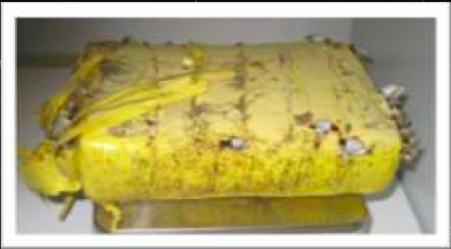
\includegraphics[width=.35\textwidth]{figures/drug1}
		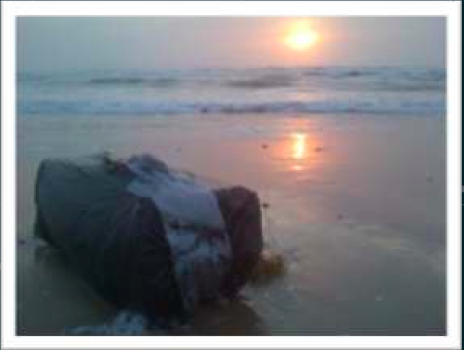
\includegraphics[width=.35\textwidth]{figures/drug2}\\
		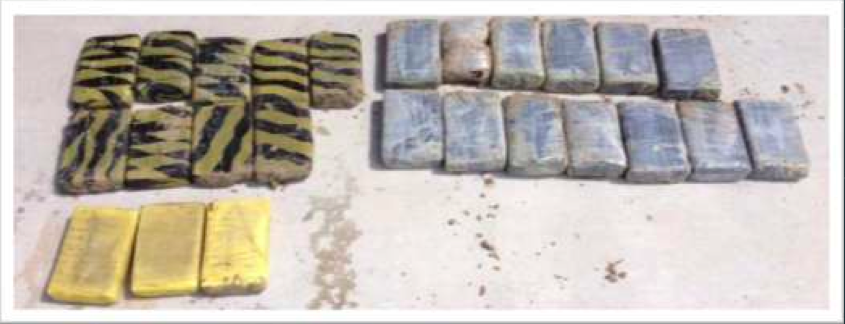
\includegraphics[width=.7\textwidth]{figures/drug3}
	\end{figure}
	\tiny{US Coast Guard District 8}
\end{frame}

\begin{frame}[t]\frametitle{Oil spill transport}    
	\begin{figure}[htbp]
		\centering
		\only<1>{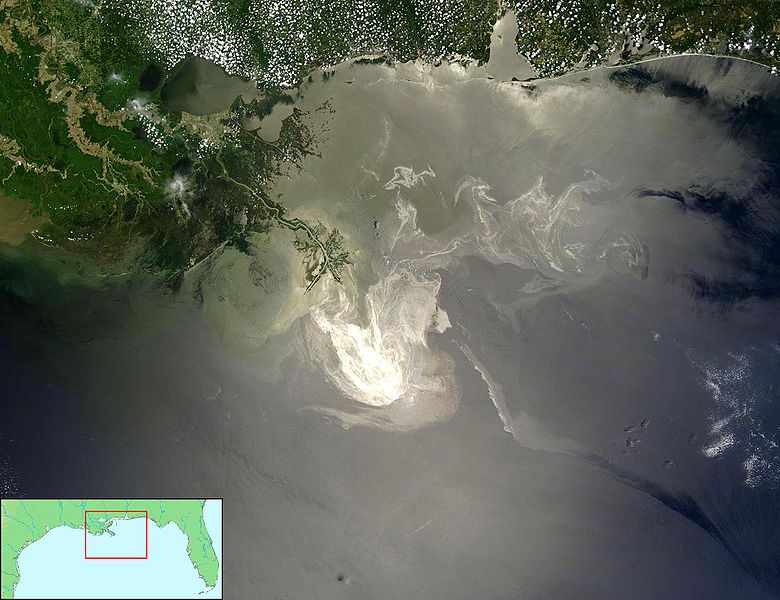
\includegraphics[width=.7\textwidth]{figures/oil}}
		\only<2>{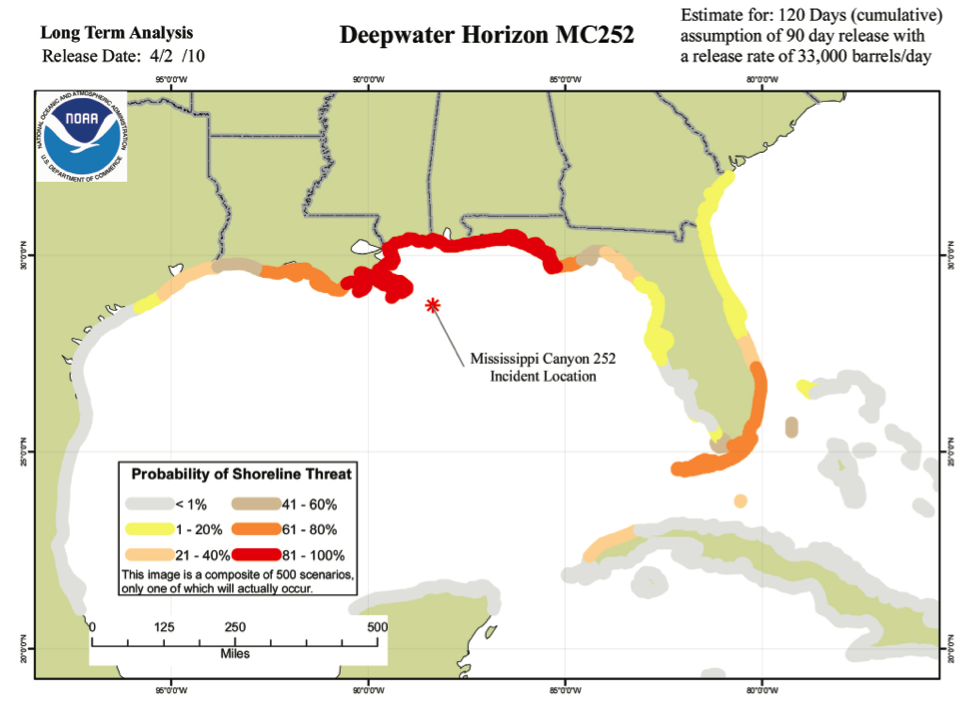
\includegraphics[width=.7\textwidth]{figures/dwh_noaa}}
	\end{figure}
	\only<1>{\tiny{NASA's Terra Satellite}}
	\only<2>{\tiny{Barker, C. H., 2005, AGU Monograph: \textit{Monitoring and Modeling the Deepwater Horizon Oil Spill: A Record-Breaking Enterprise}}}
\end{frame}

\begin{frame}
	\frametitle{Harmful Algal Bloom Events in Texas Waters}
	\begin{figure}[htbp]
		\centering
		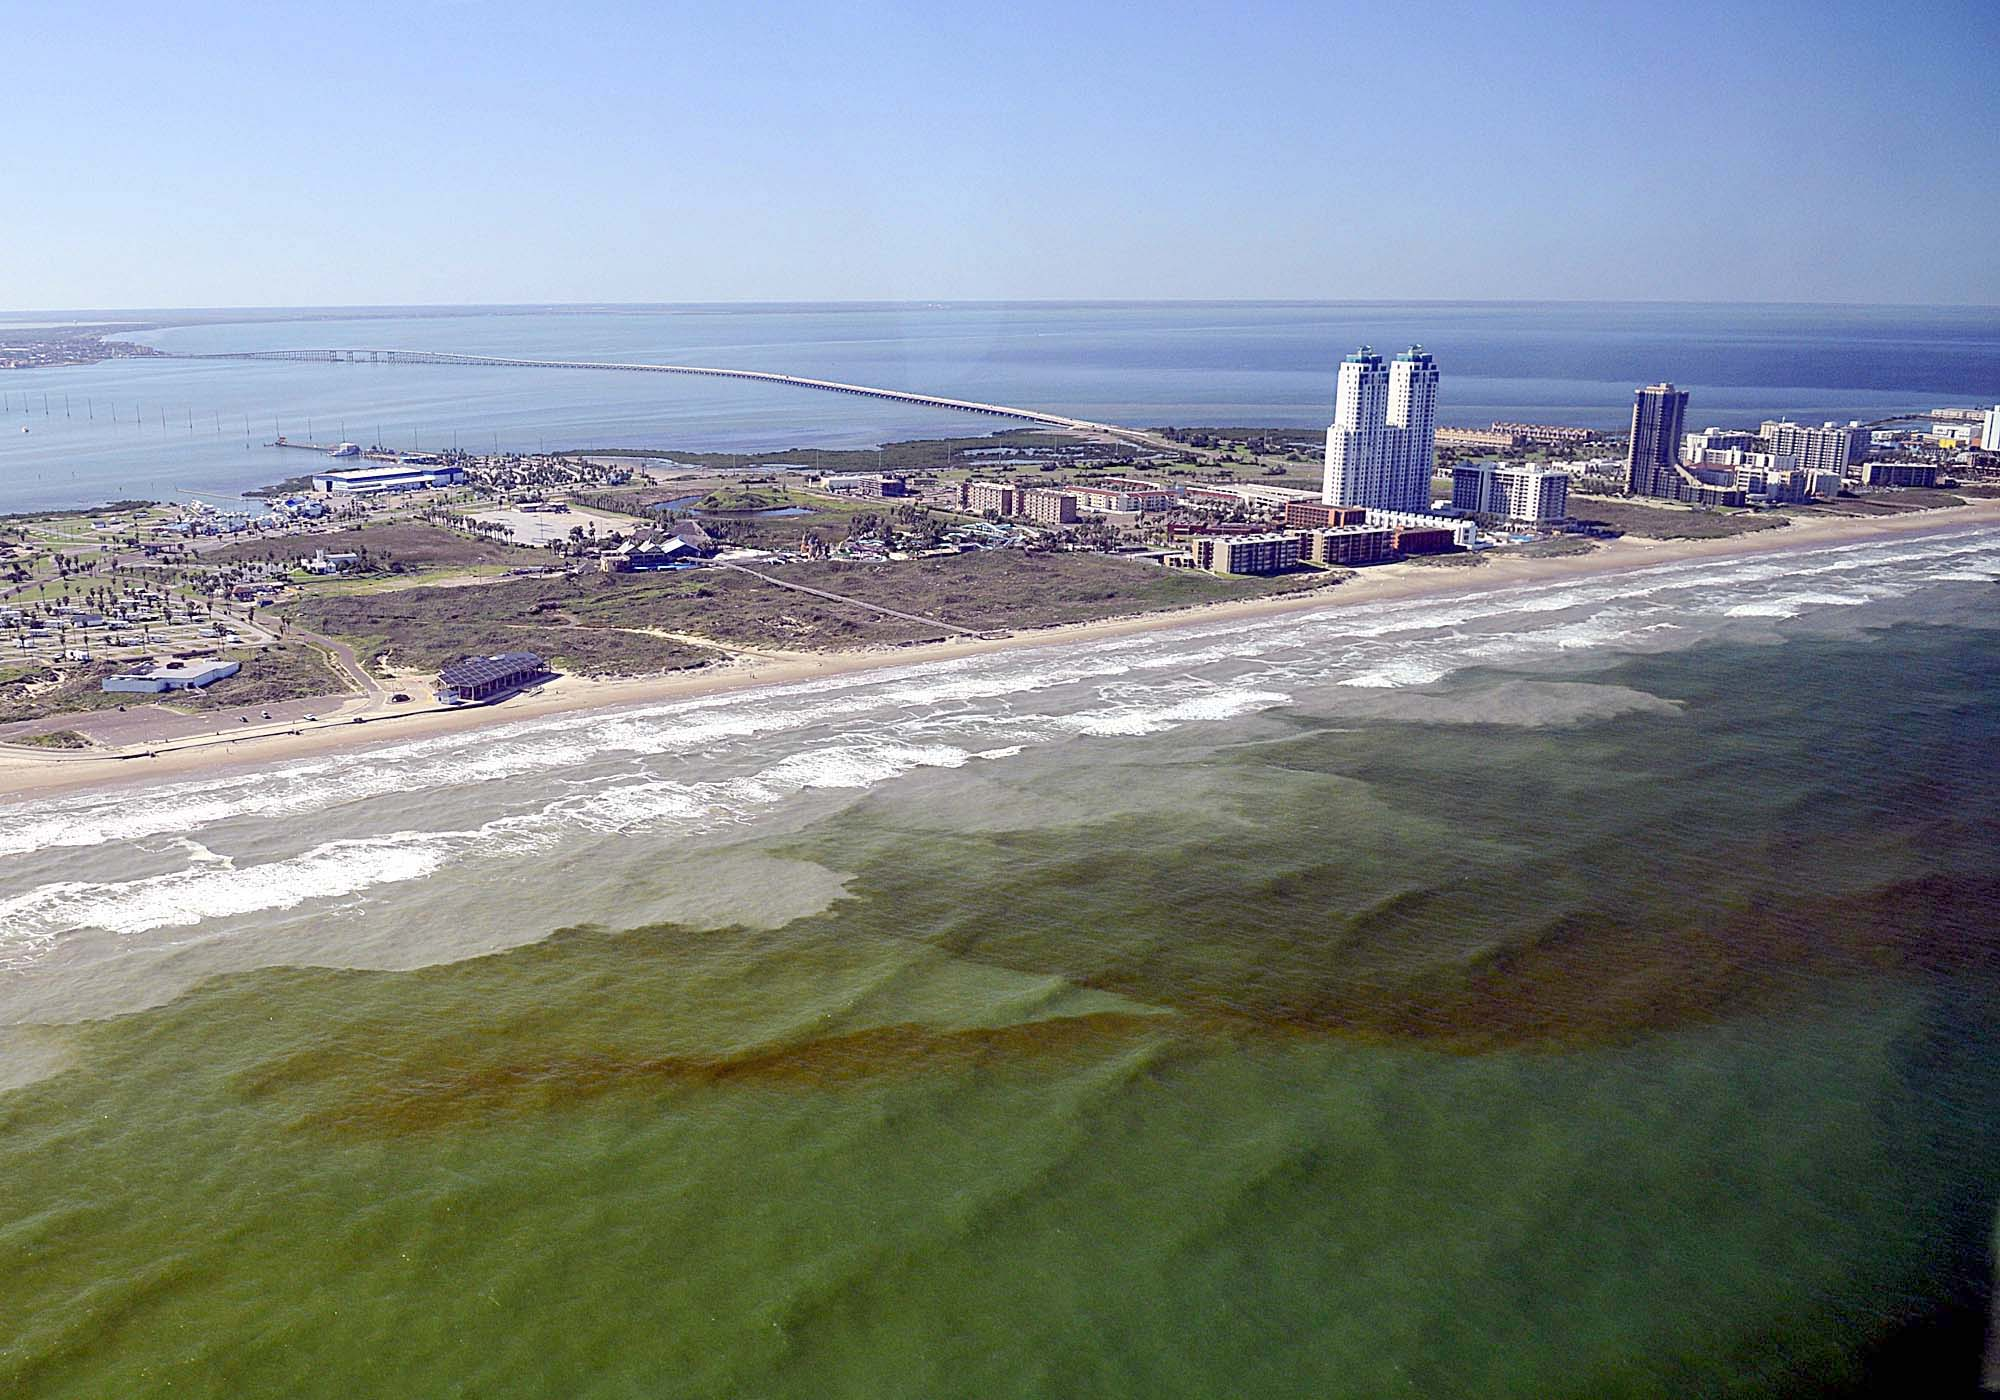
\includegraphics[width=0.8\textwidth]{figures/Red_Tide_SPI_3632}
	\end{figure}
	\vskip2ex
	{\tiny Photo: Texas Parks and Wildlife Department}
\end{frame}

\begin{frame}
	\frametitle{Lagrangian Approach to Understanding HABs}
	\begin{figure}[htbp]
		\centering
		\only<1>{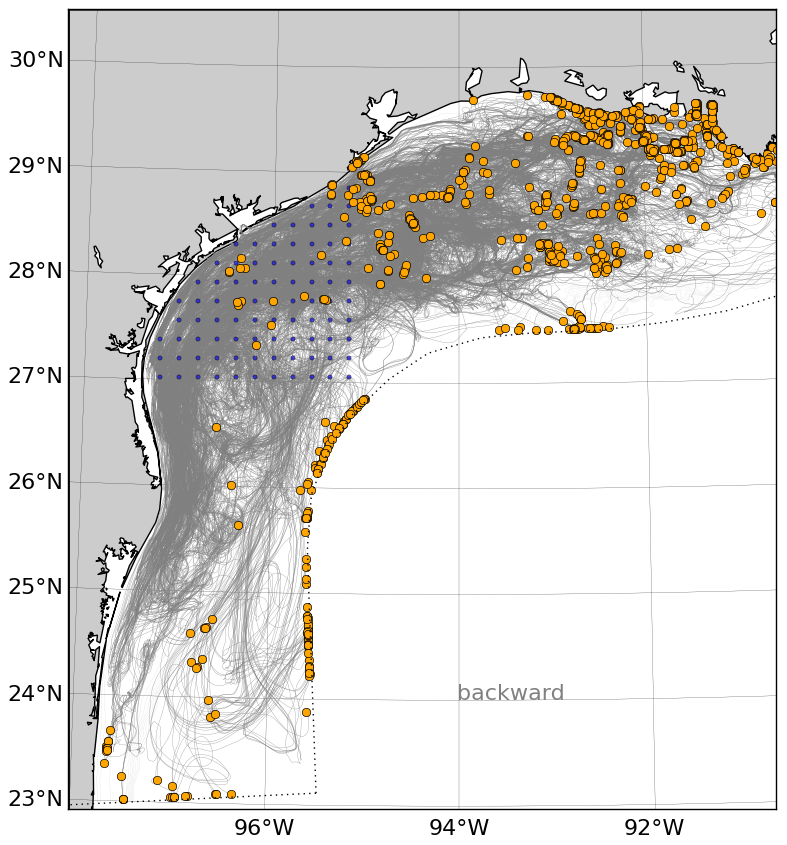
\includegraphics[width=.5\textwidth]{figures/exp7_example}}
		\only<2>{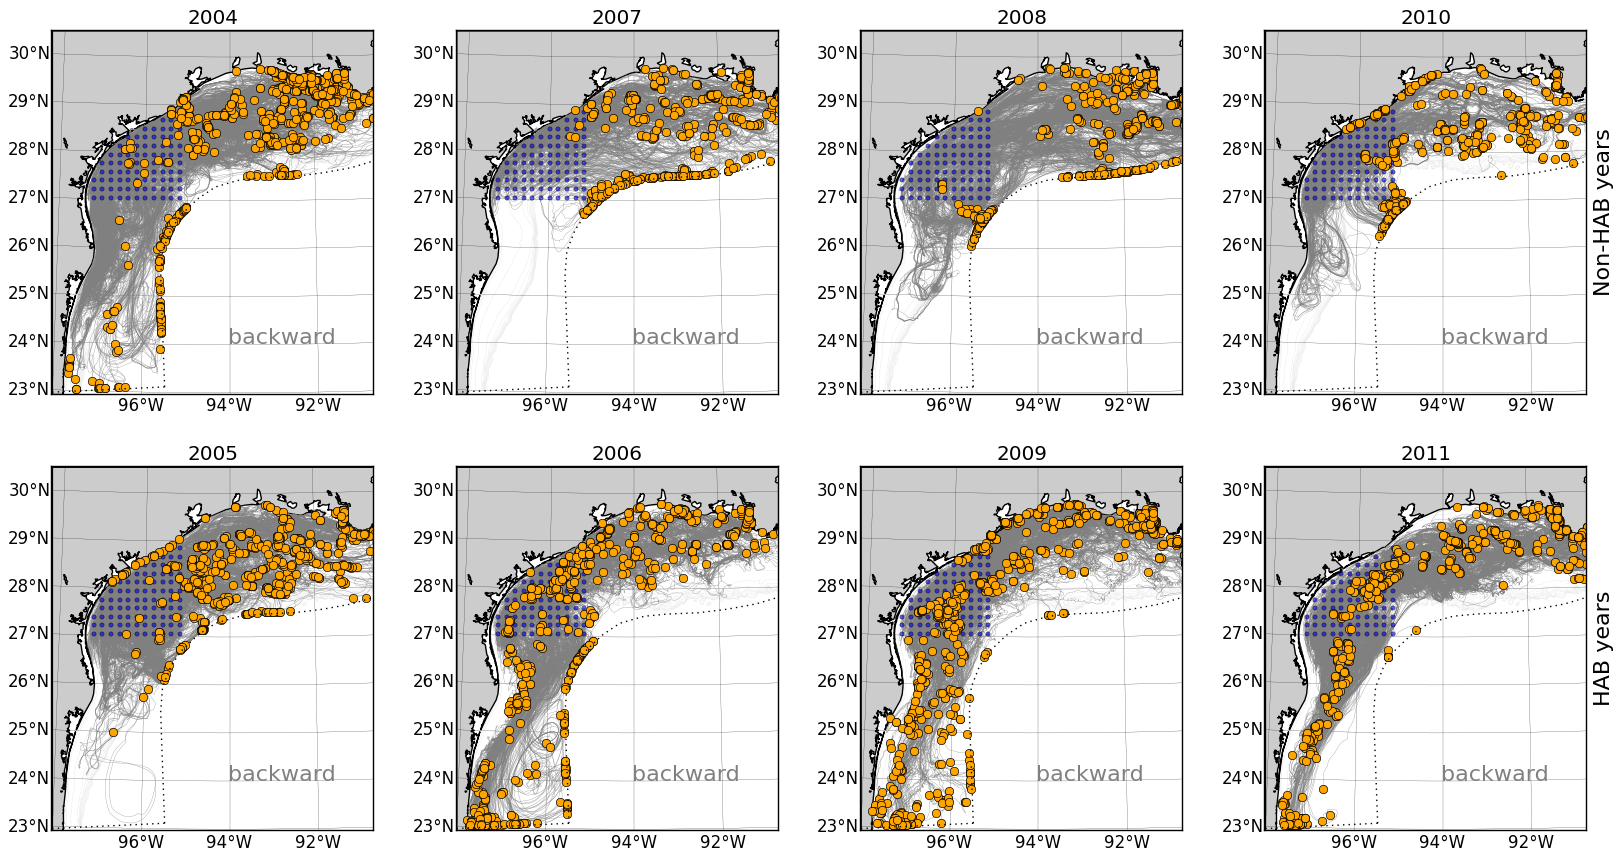
\includegraphics[width=\textwidth]{figures/exp70901}}
		% \only<3>{\includegraphics[width=\textwidth]{figures/exp20925PAtracks09}}
		% \only<3>{\includegraphics[width=\textwidth]{figures/conByHAB0601hexbin}}
	\end{figure}
	{\tiny Thyng, K.M, et al, L\&O:FE 2013}
	% \only<2>{Tracking drifters backward from Port Aransas from the autumn into summer helps indicate their origin}
	% \only<3>{Drifters always come from the east, but tend to also come from the south in HAB years}
\end{frame}


%%% Numerical Approach %%%

\section{Numerical Approach}


% \begin{frame}[t]\frametitle{Numerical Approach}
%     Describe model domain, features and setup of model, some validation


% \end{frame}

\begin{frame}[t]\frametitle{Numerical Domain}
	\begin{figure}[htbp]
		\centering
		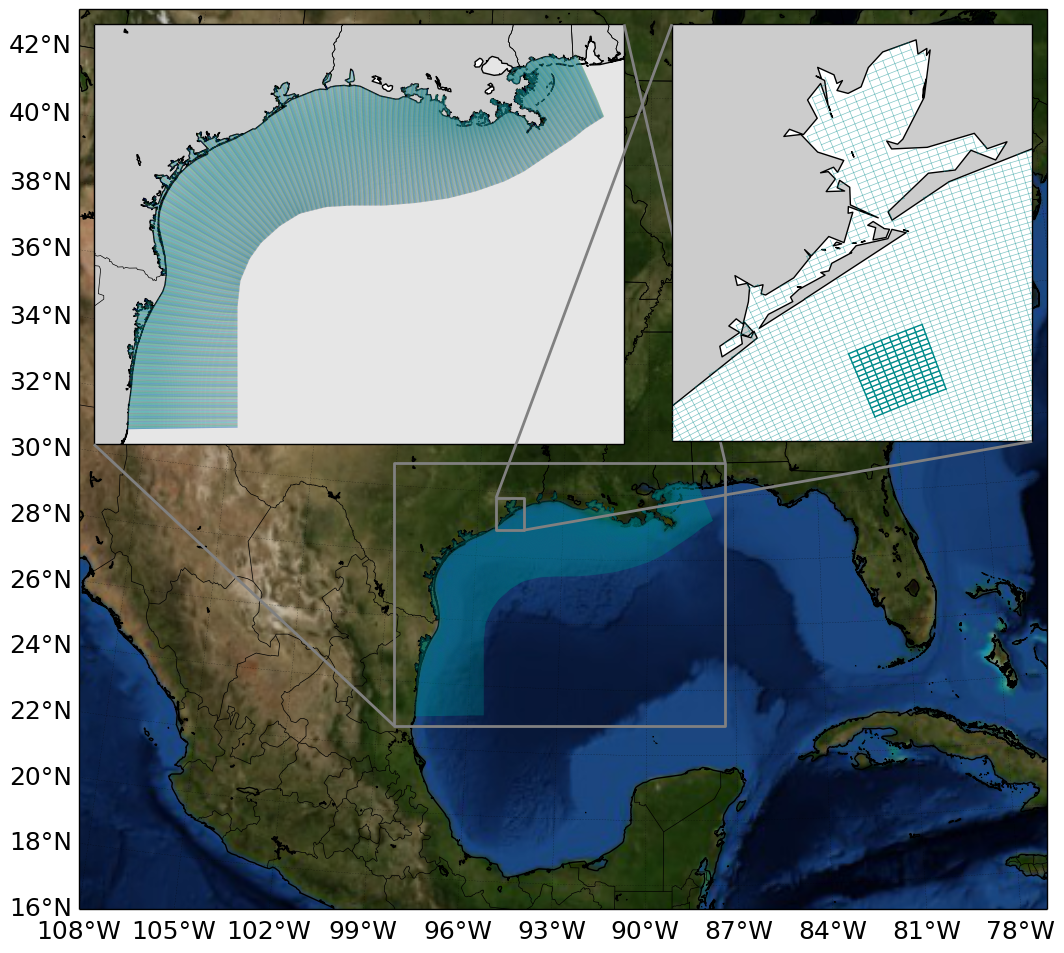
\includegraphics[width=0.6\textwidth]{figures/TXLA_domain.png}
	\end{figure}
\end{frame}


\begin{frame}[t]\frametitle{Surface Salinity}
	\begin{figure}
	  	\centering
	   	\includemovie[autoplay, poster, autopause, autoresume, controls, repeat
	   	]{\textwidth}{0.4\textwidth}{figures/2008.mp4}
		%\vskip-1ex
	\end{figure}
\end{frame}

\begin{frame}[t]\frametitle{TRACMASS}
	\begin{figure}[htbp]
		\centering
		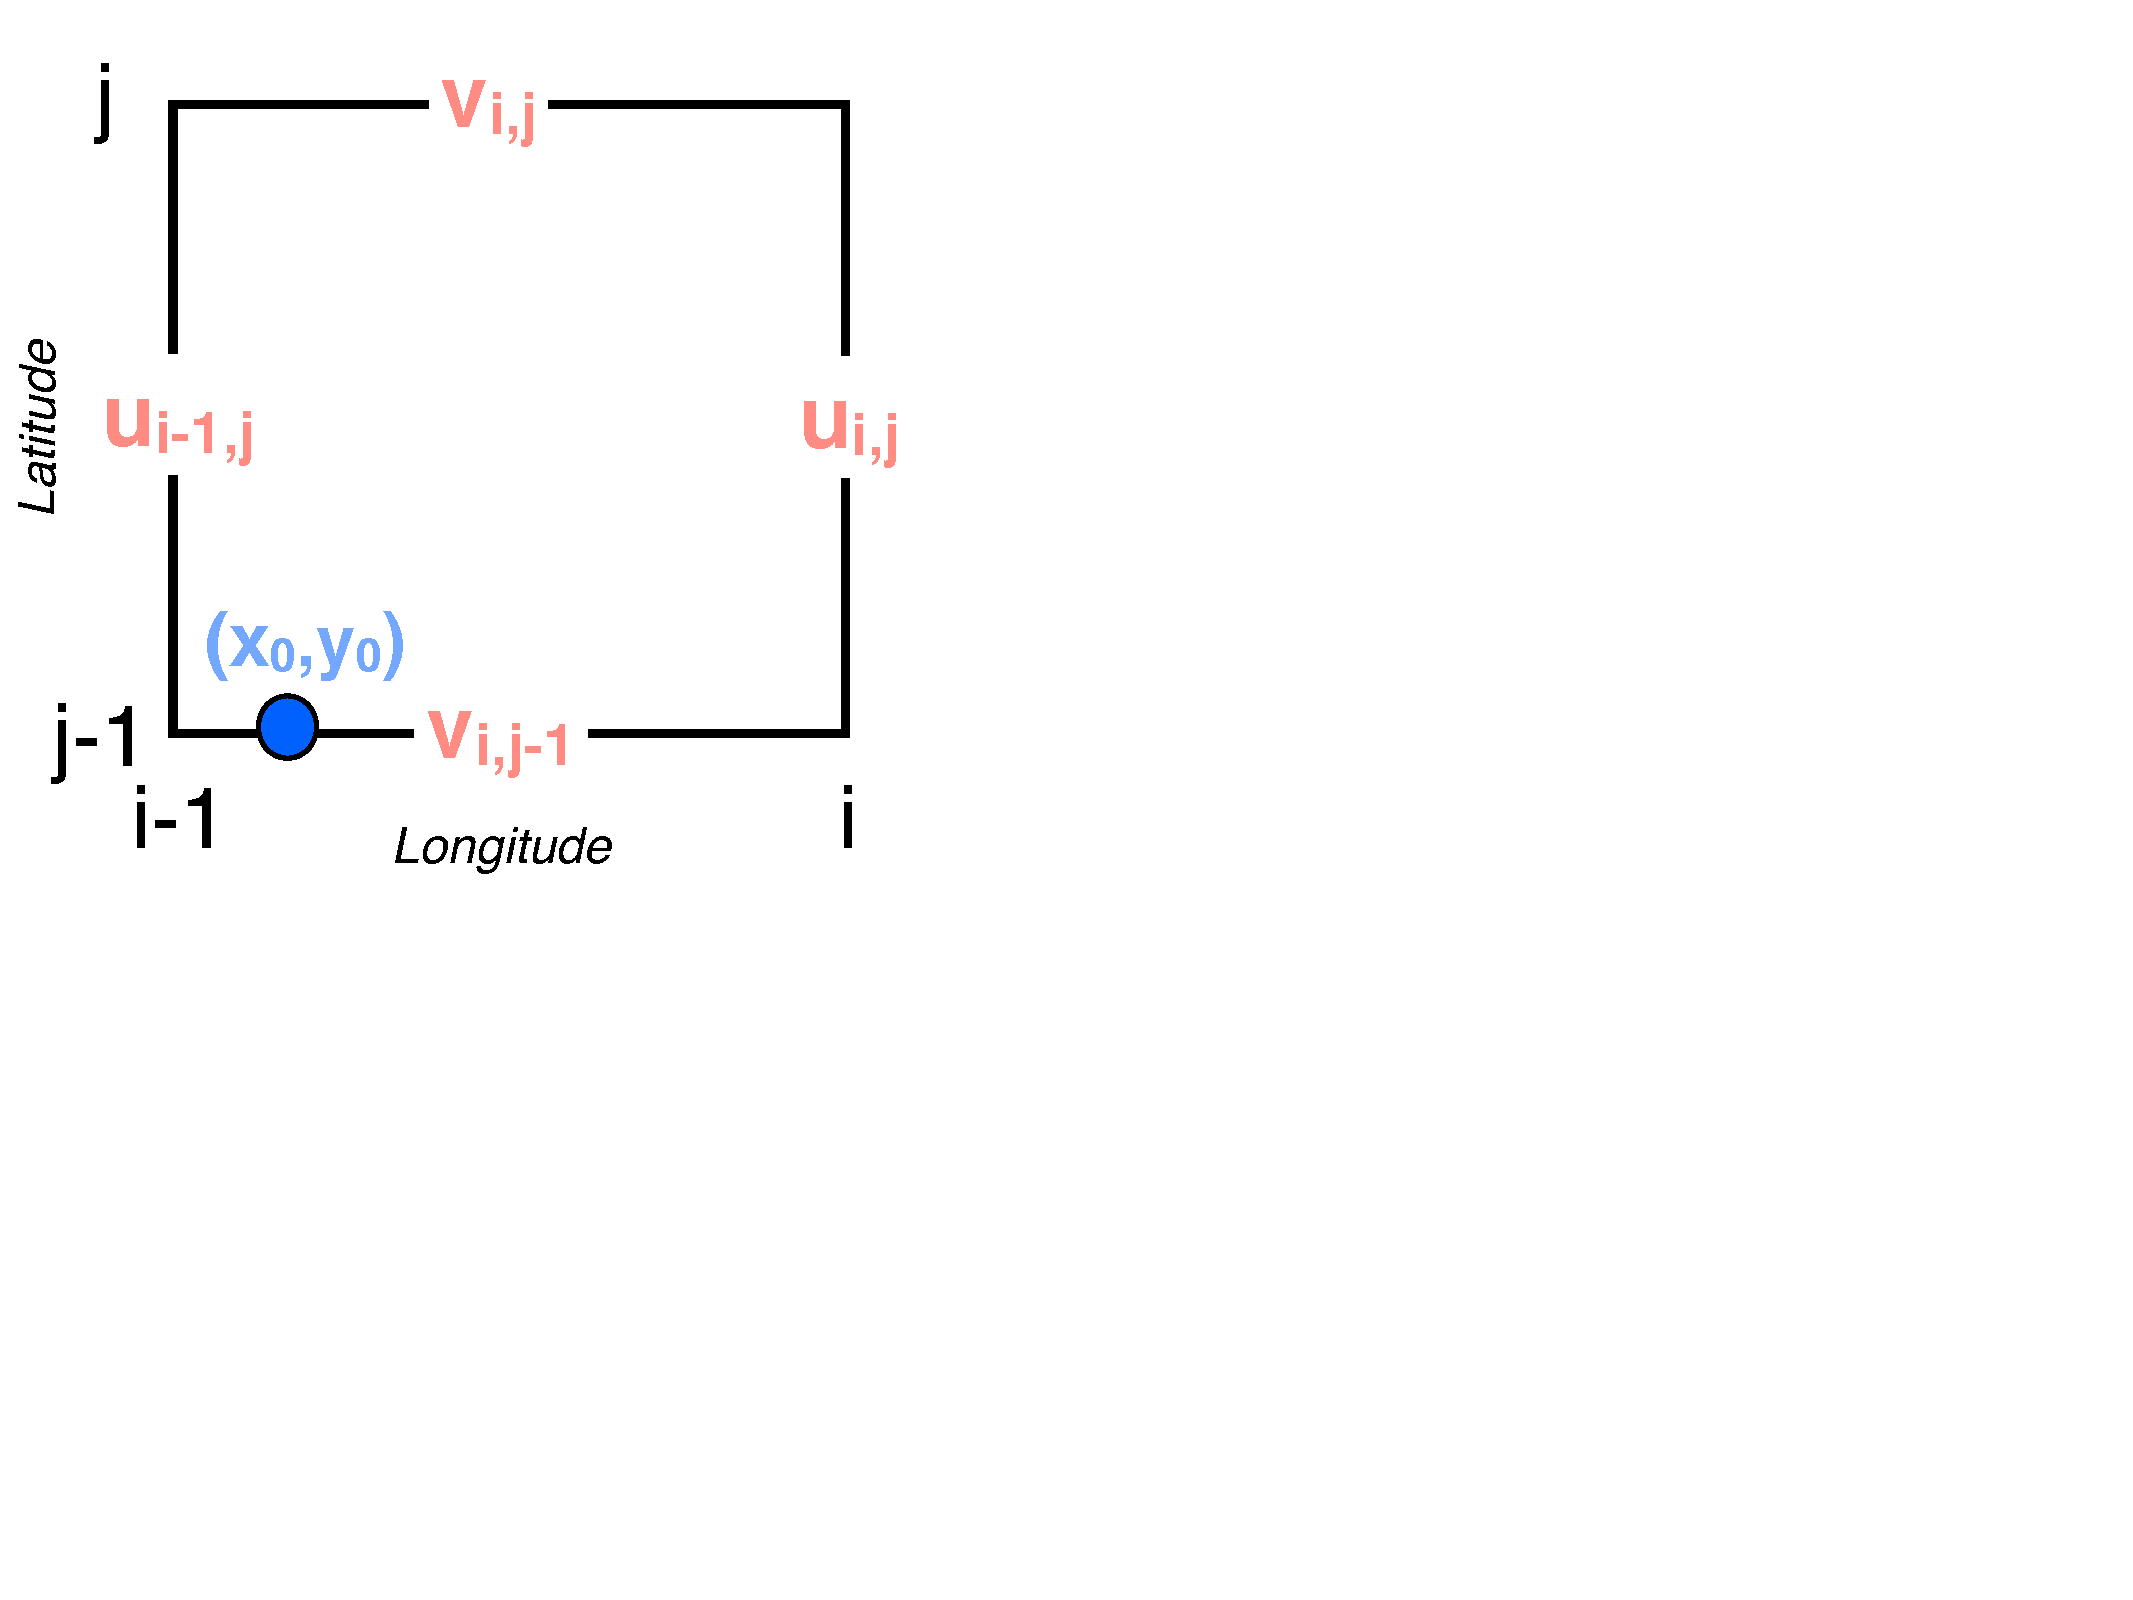
\includegraphics[width=.5\textwidth]{figures/tracmass_box1}
	\end{figure}
	{\Large Horizontal velocities on a staggered Arakawa C grid}
	\tiny{\\After TRACMASS documentation. http://www.tracmass.org, http://doos.misu.su.se/tracmass/}
\end{frame}
\begin{frame}[t,noframenumbering]\frametitle{Lagrangian Trajectory Model}
	\begin{figure}[htbp]
		\centering
		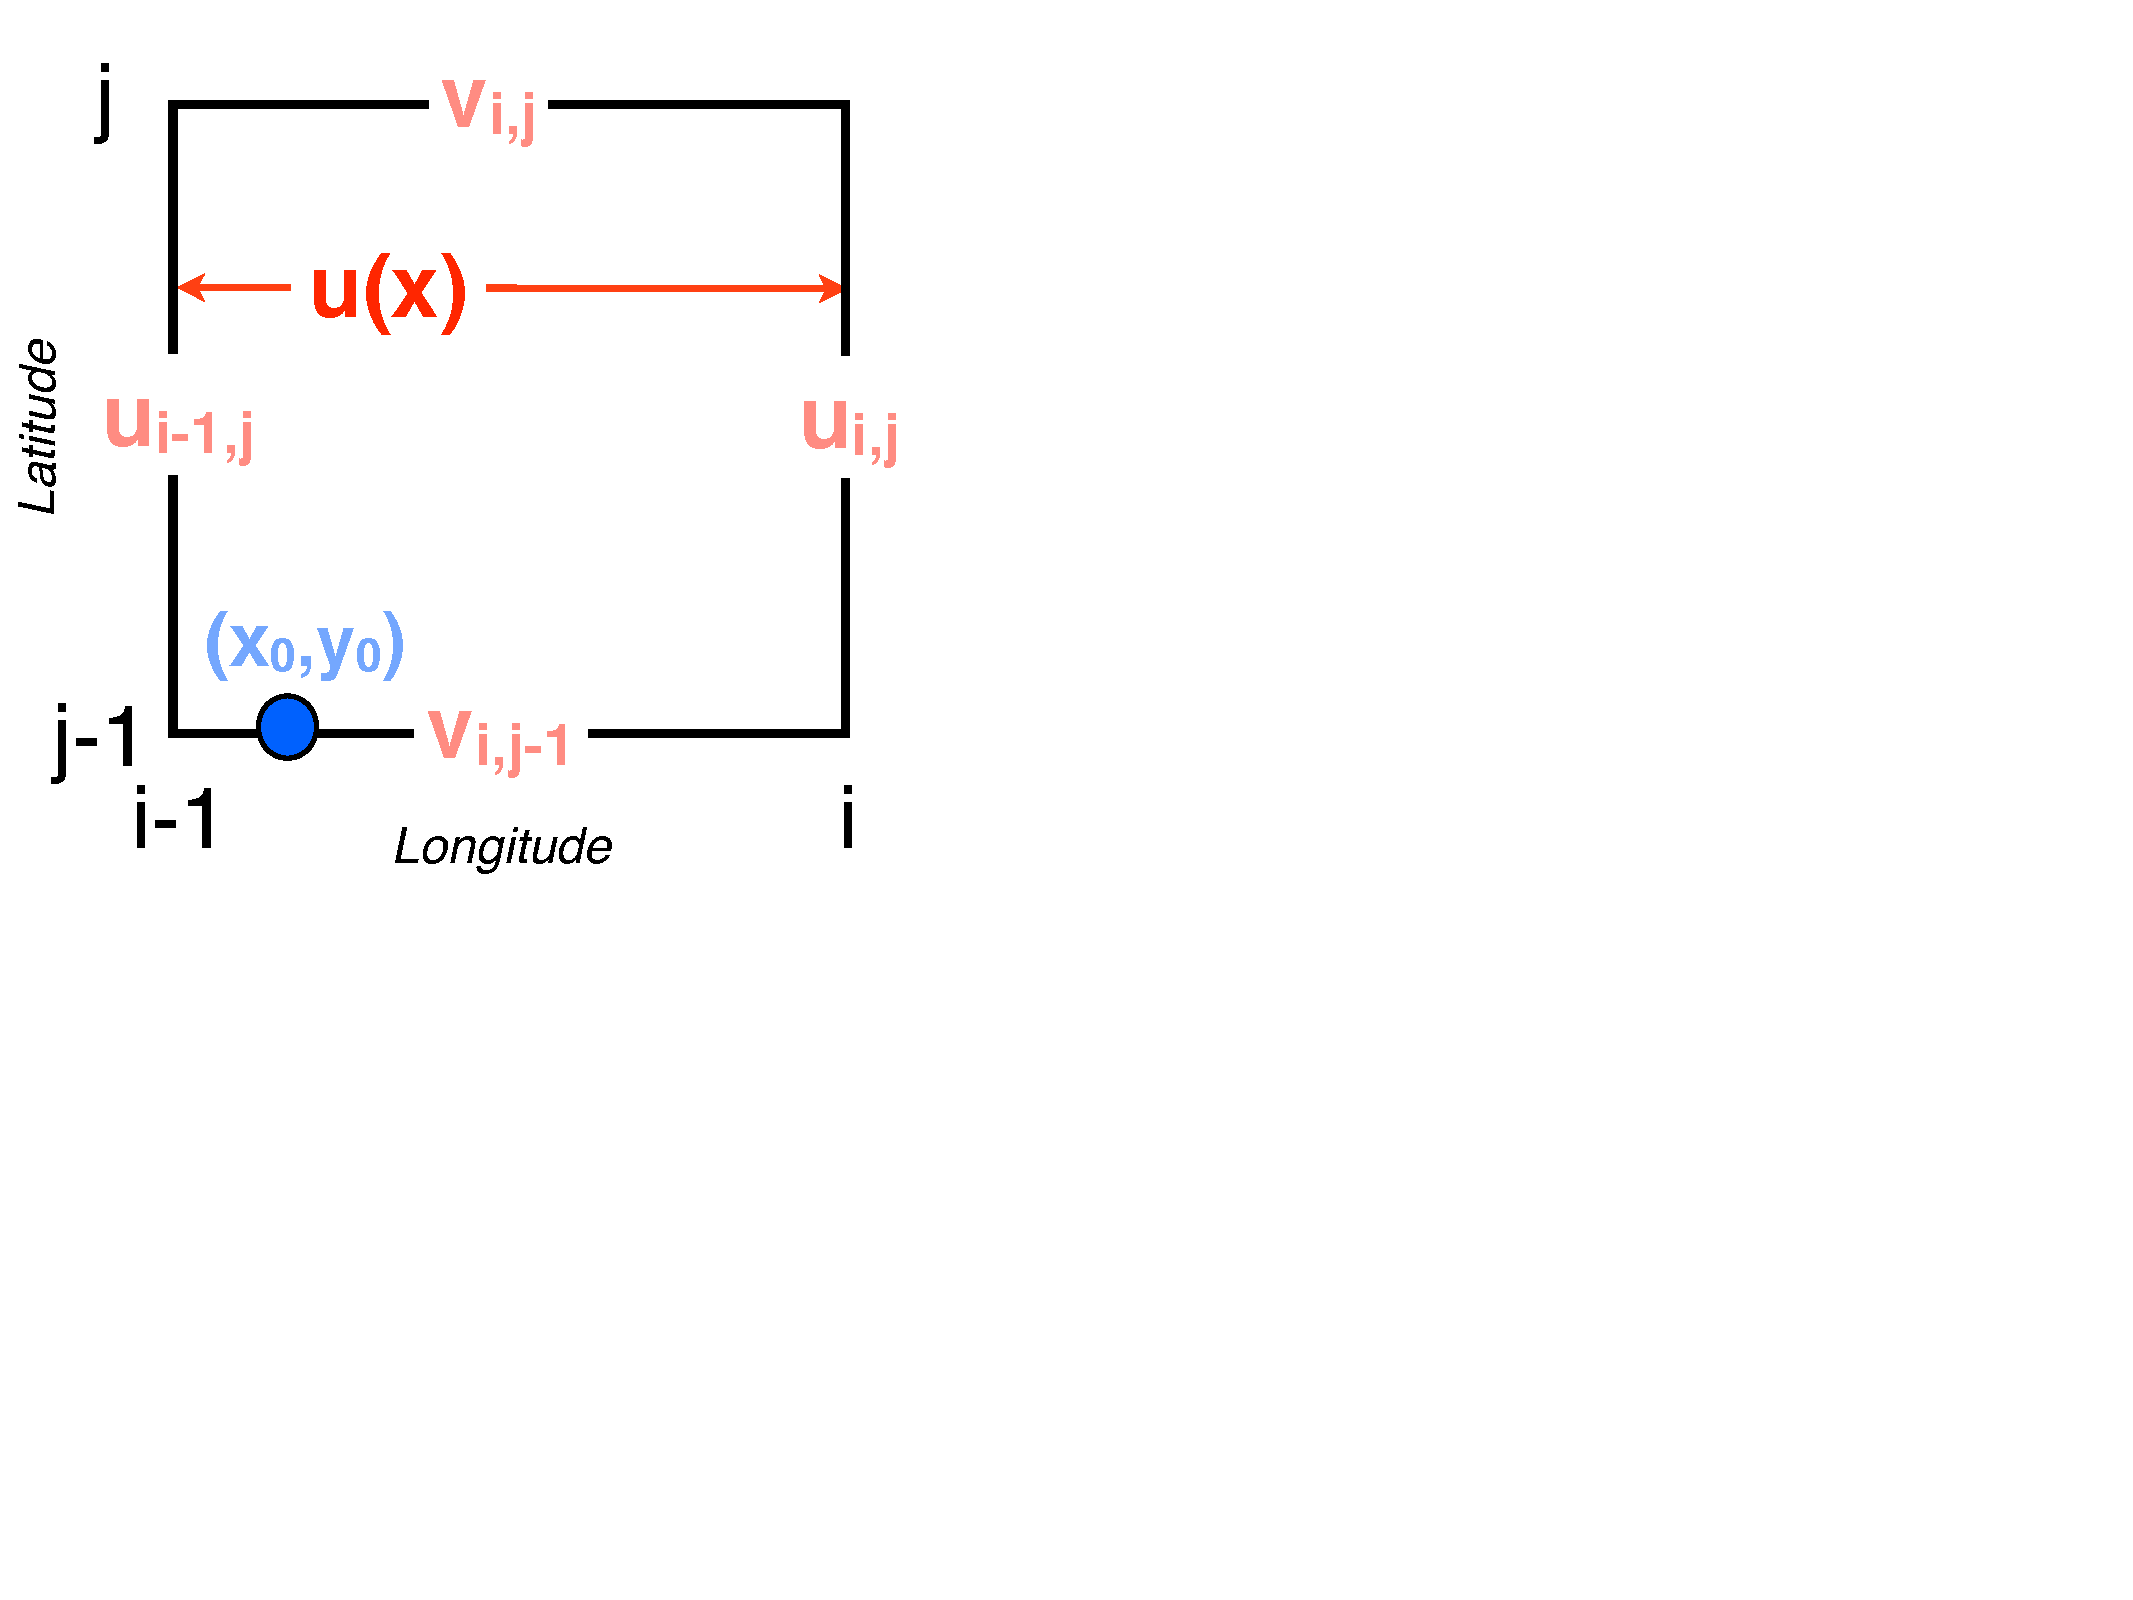
\includegraphics[width=.5\textwidth]{figures/tracmass_box2}
	\end{figure}
	{\Large Linearly interpolate $u$ in x to find $u(x)$ across cell}
	\tiny{\\After TRACMASS documentation. http://www.tracmass.org, http://doos.misu.su.se/tracmass/}
\end{frame}
\begin{frame}[t,noframenumbering]\frametitle{Lagrangian Trajectory Model}
	\begin{figure}[htbp]
		\centering
		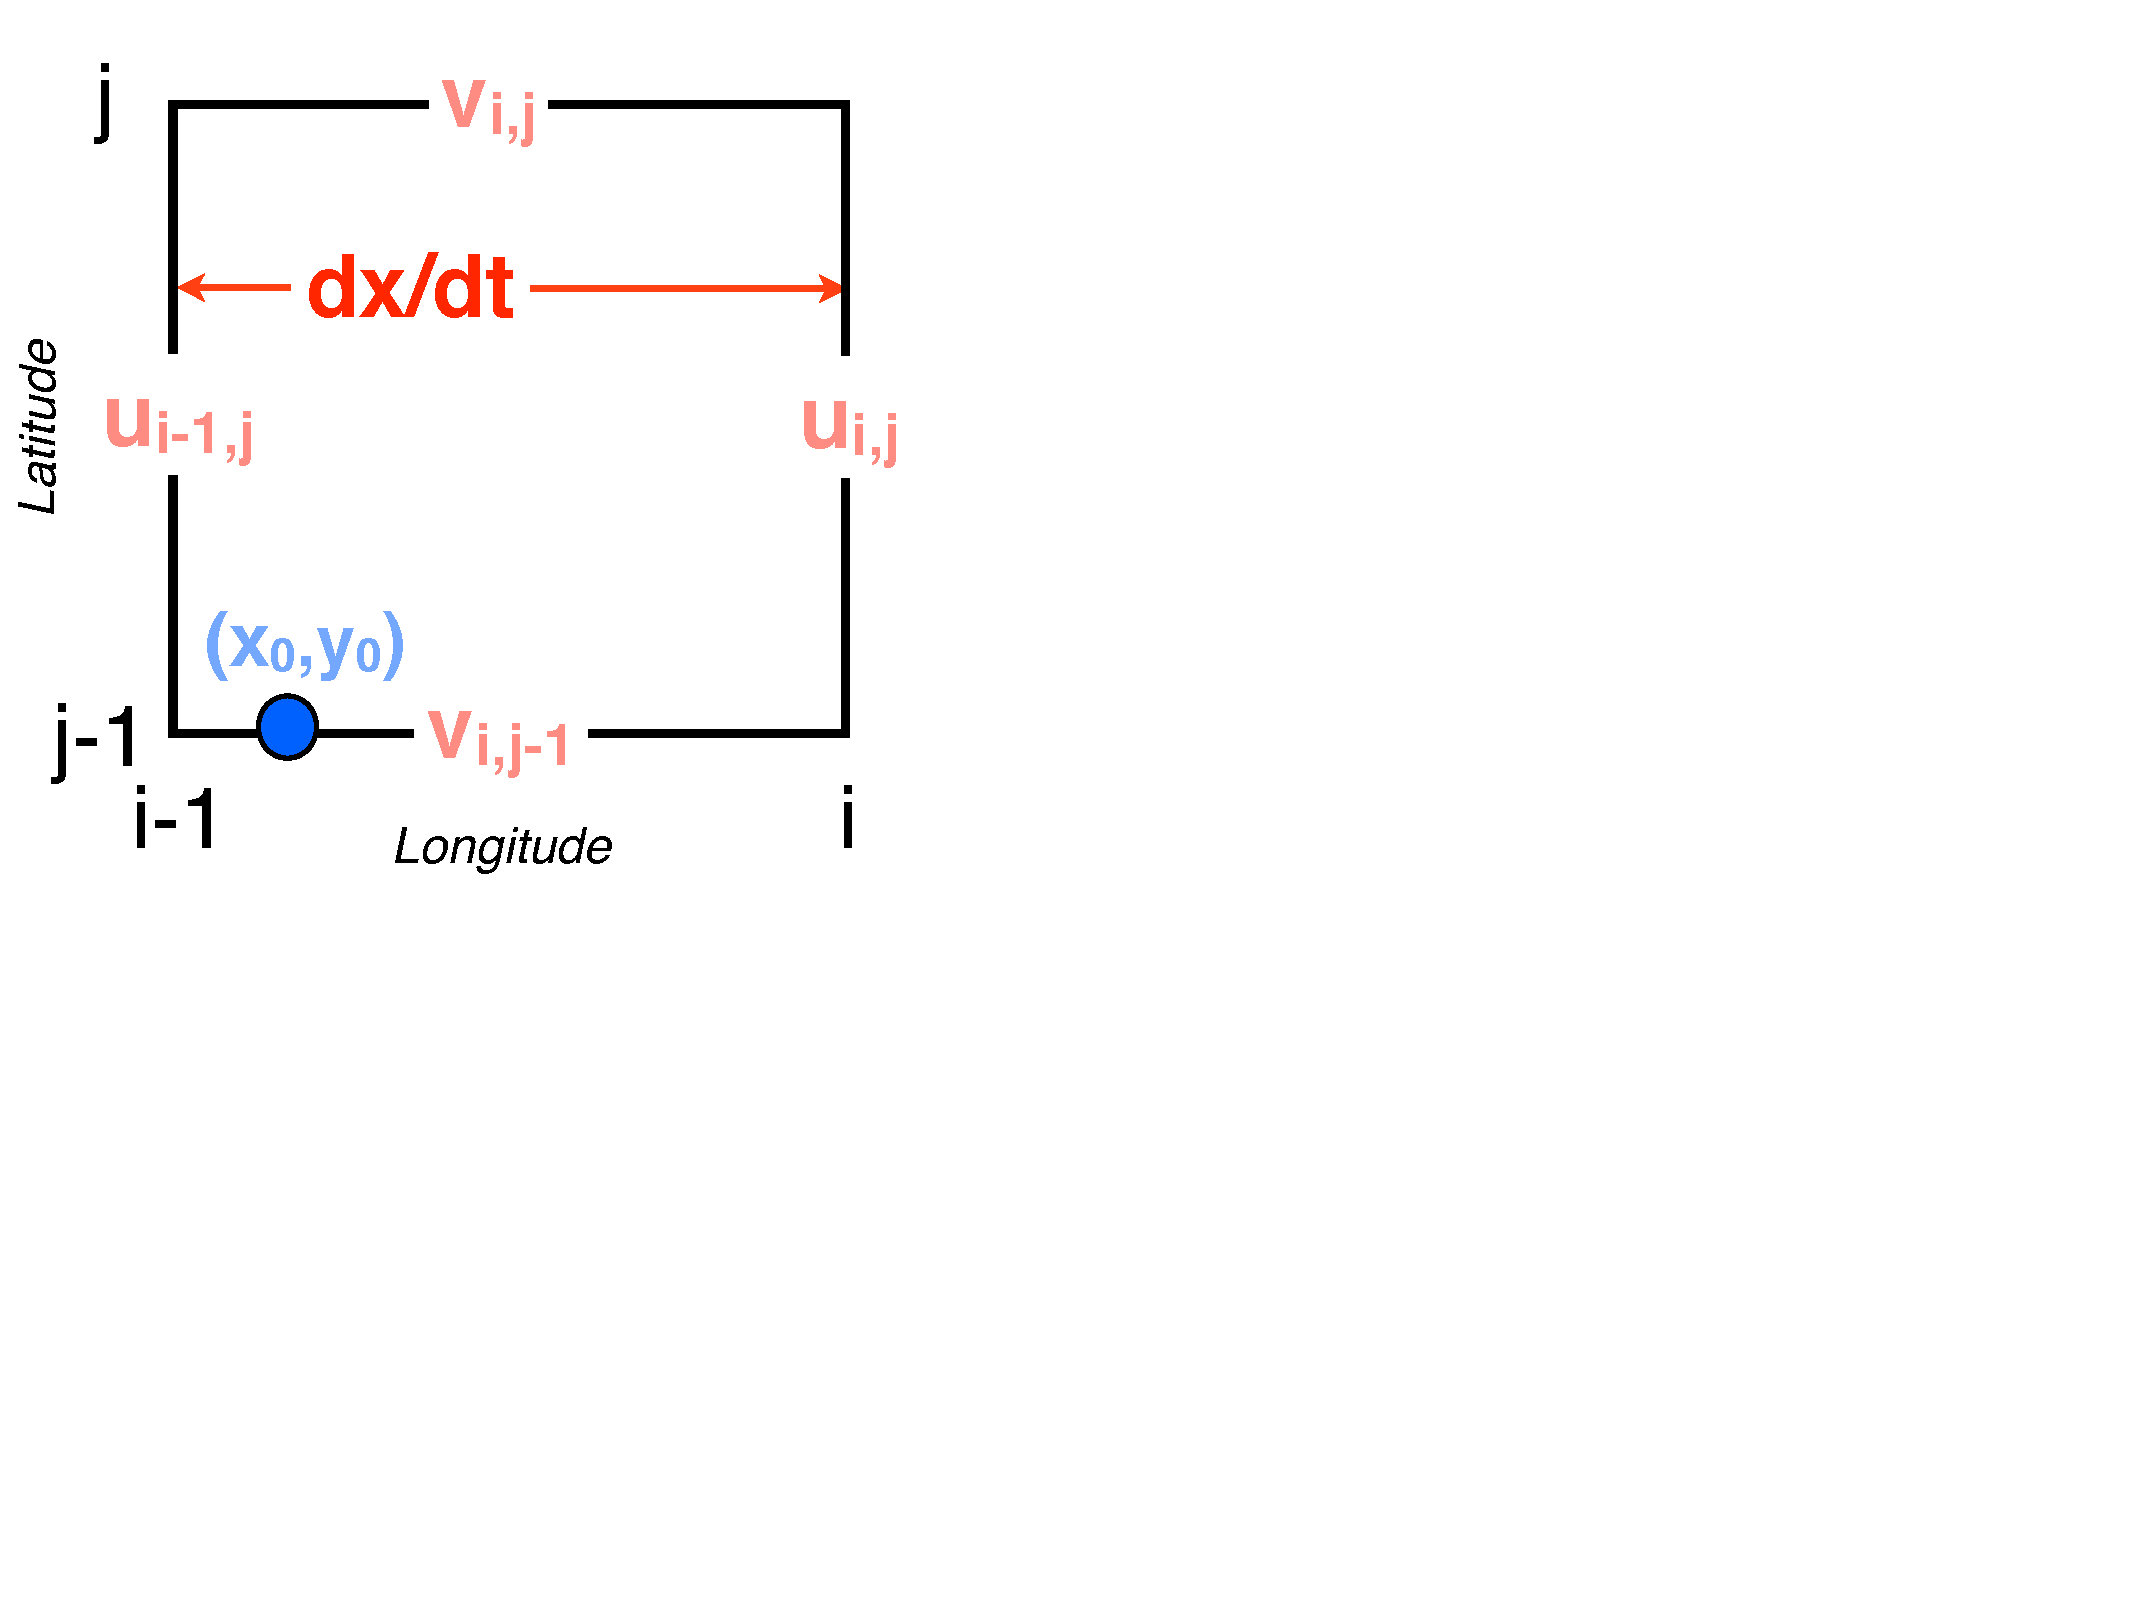
\includegraphics[width=.5\textwidth]{figures/tracmass_box3}
	\end{figure}
	{\Large $u=\frac{dx}{dt}$}
	\tiny{\\After TRACMASS documentation. http://www.tracmass.org, http://doos.misu.su.se/tracmass/}
\end{frame}
\begin{frame}[t,noframenumbering]\frametitle{Lagrangian Trajectory Model}
	\begin{figure}[htbp]
		\centering
		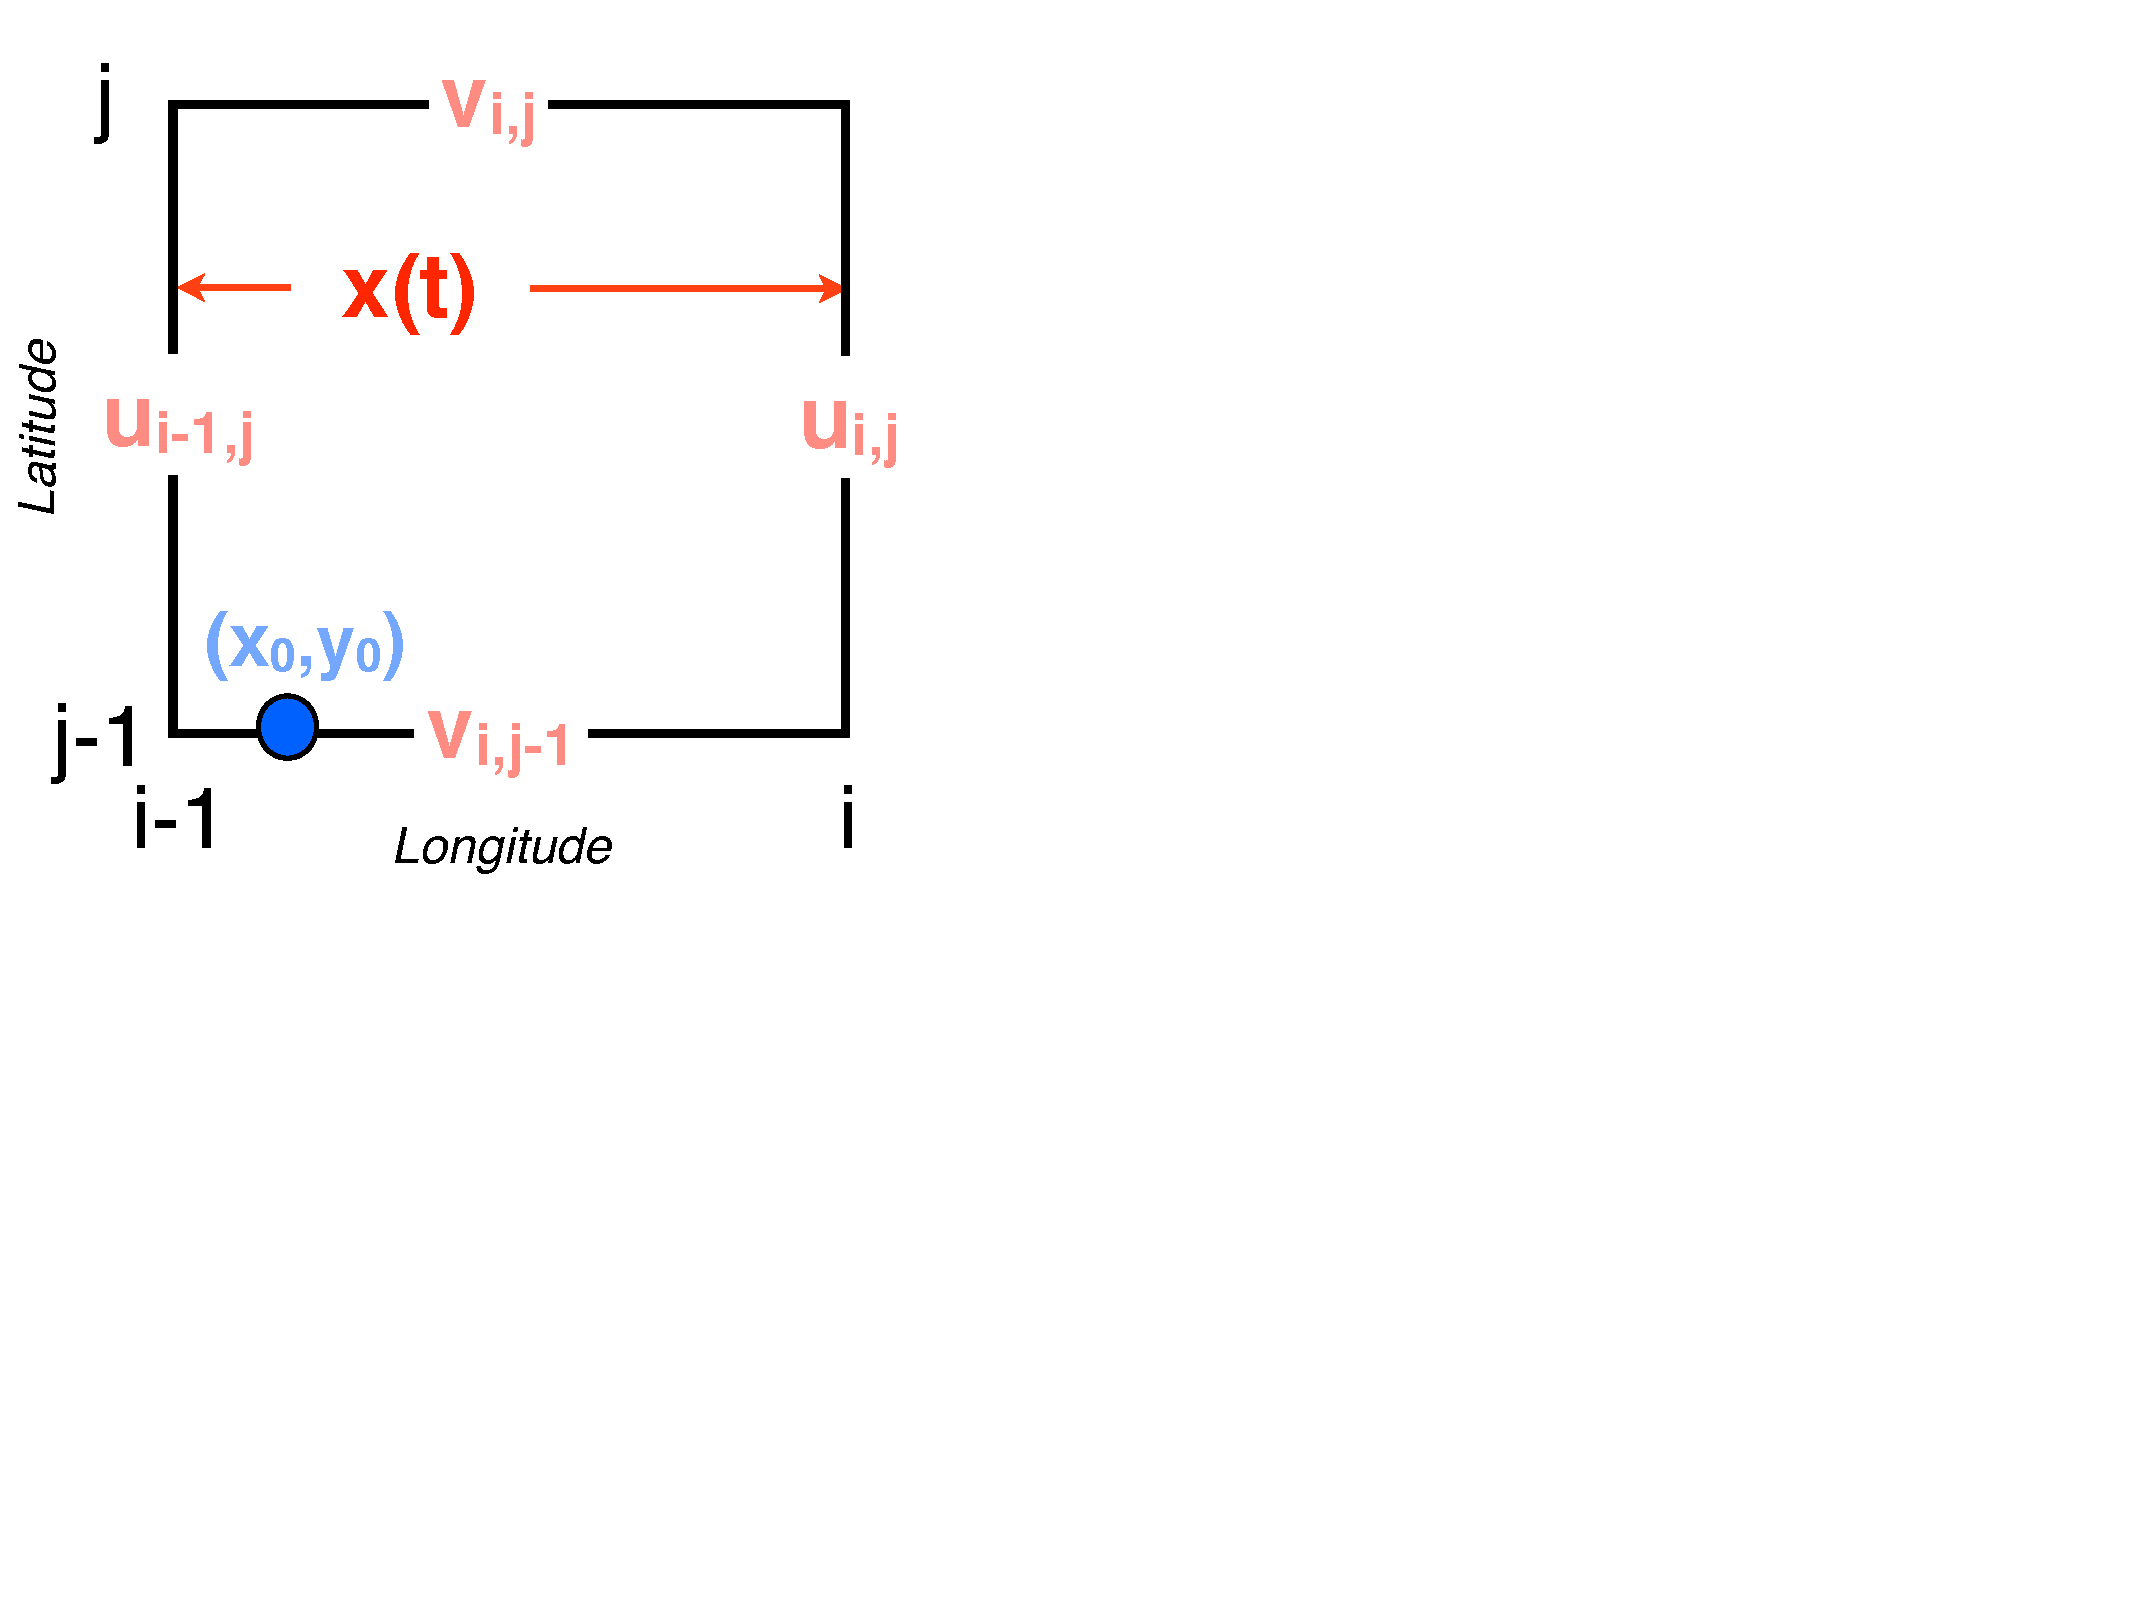
\includegraphics[width=.5\textwidth]{figures/tracmass_box4}
	\end{figure}
	{\Large $\frac{dx}{dt}$ can be analytically solved for $x(t)$}
	\tiny{\\After TRACMASS documentation. http://www.tracmass.org, http://doos.misu.su.se/tracmass/}
\end{frame}
\begin{frame}[t,noframenumbering]\frametitle{Lagrangian Trajectory Model}
	\begin{figure}[htbp]
		\centering
		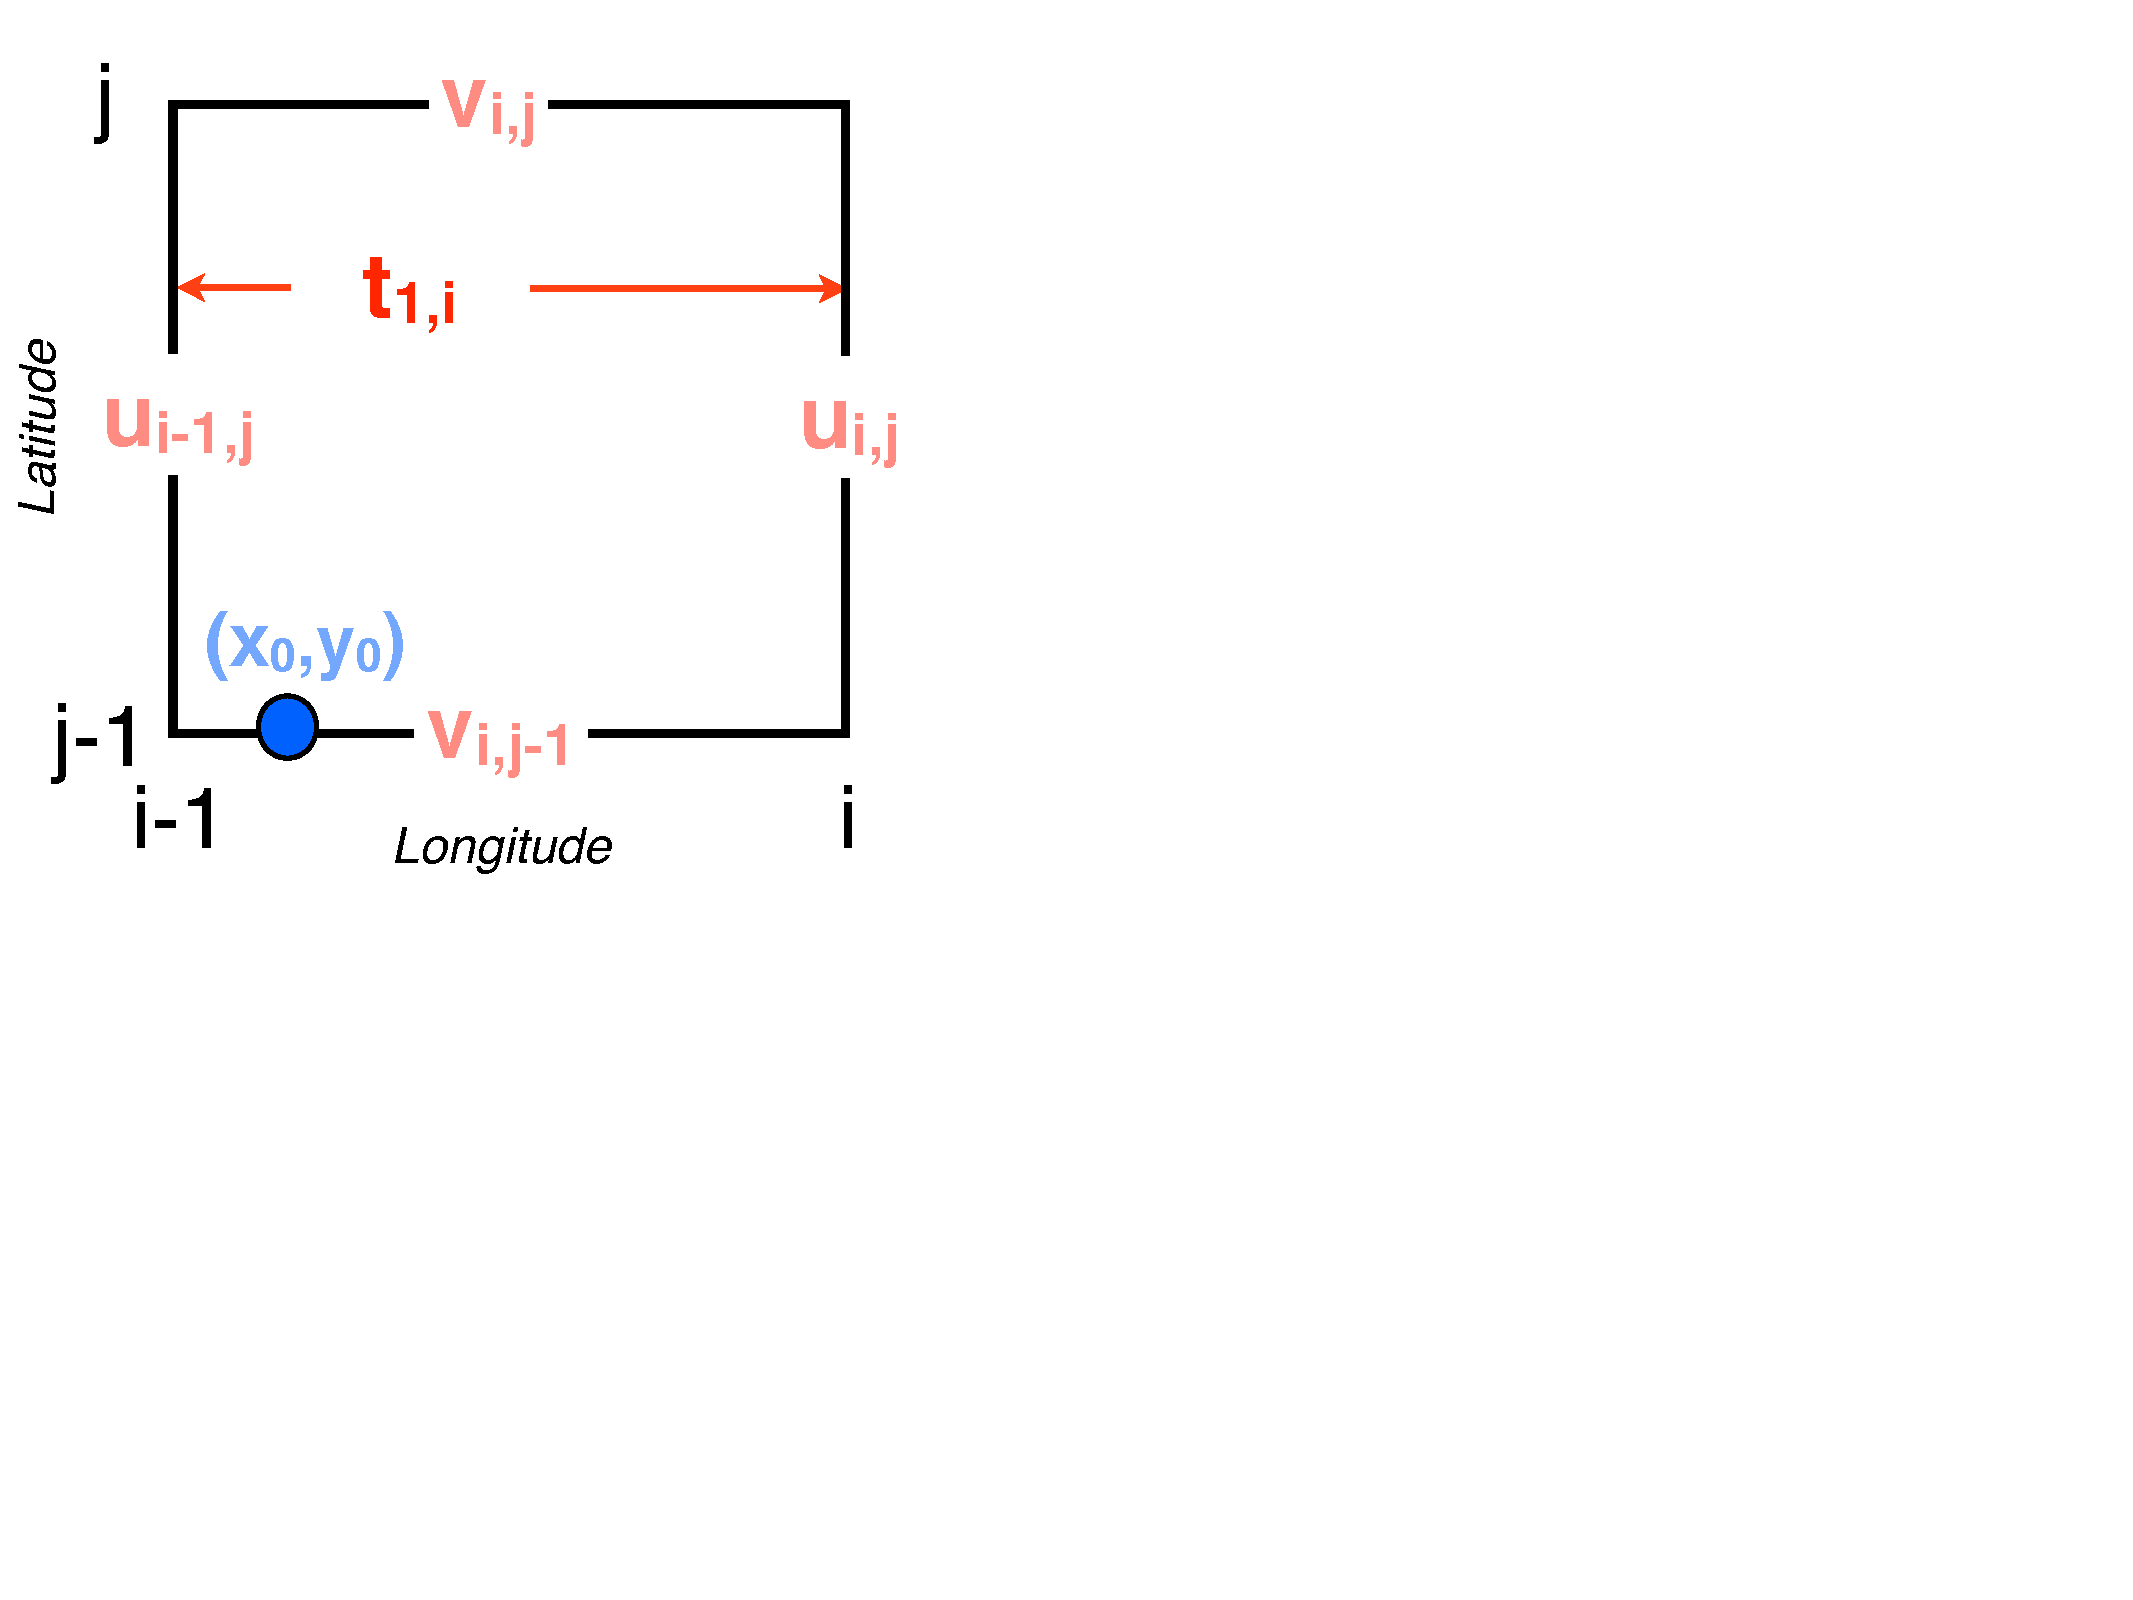
\includegraphics[width=.5\textwidth]{figures/tracmass_box5}
	\end{figure}
	{\Large Solve for the time $t$ when drifter would hit $x$ wall}
	\tiny{\\After TRACMASS documentation. http://www.tracmass.org, http://doos.misu.su.se/tracmass/}
\end{frame}
\begin{frame}[t,noframenumbering]\frametitle{Lagrangian Trajectory Model}
	\begin{figure}[htbp]
		\centering
		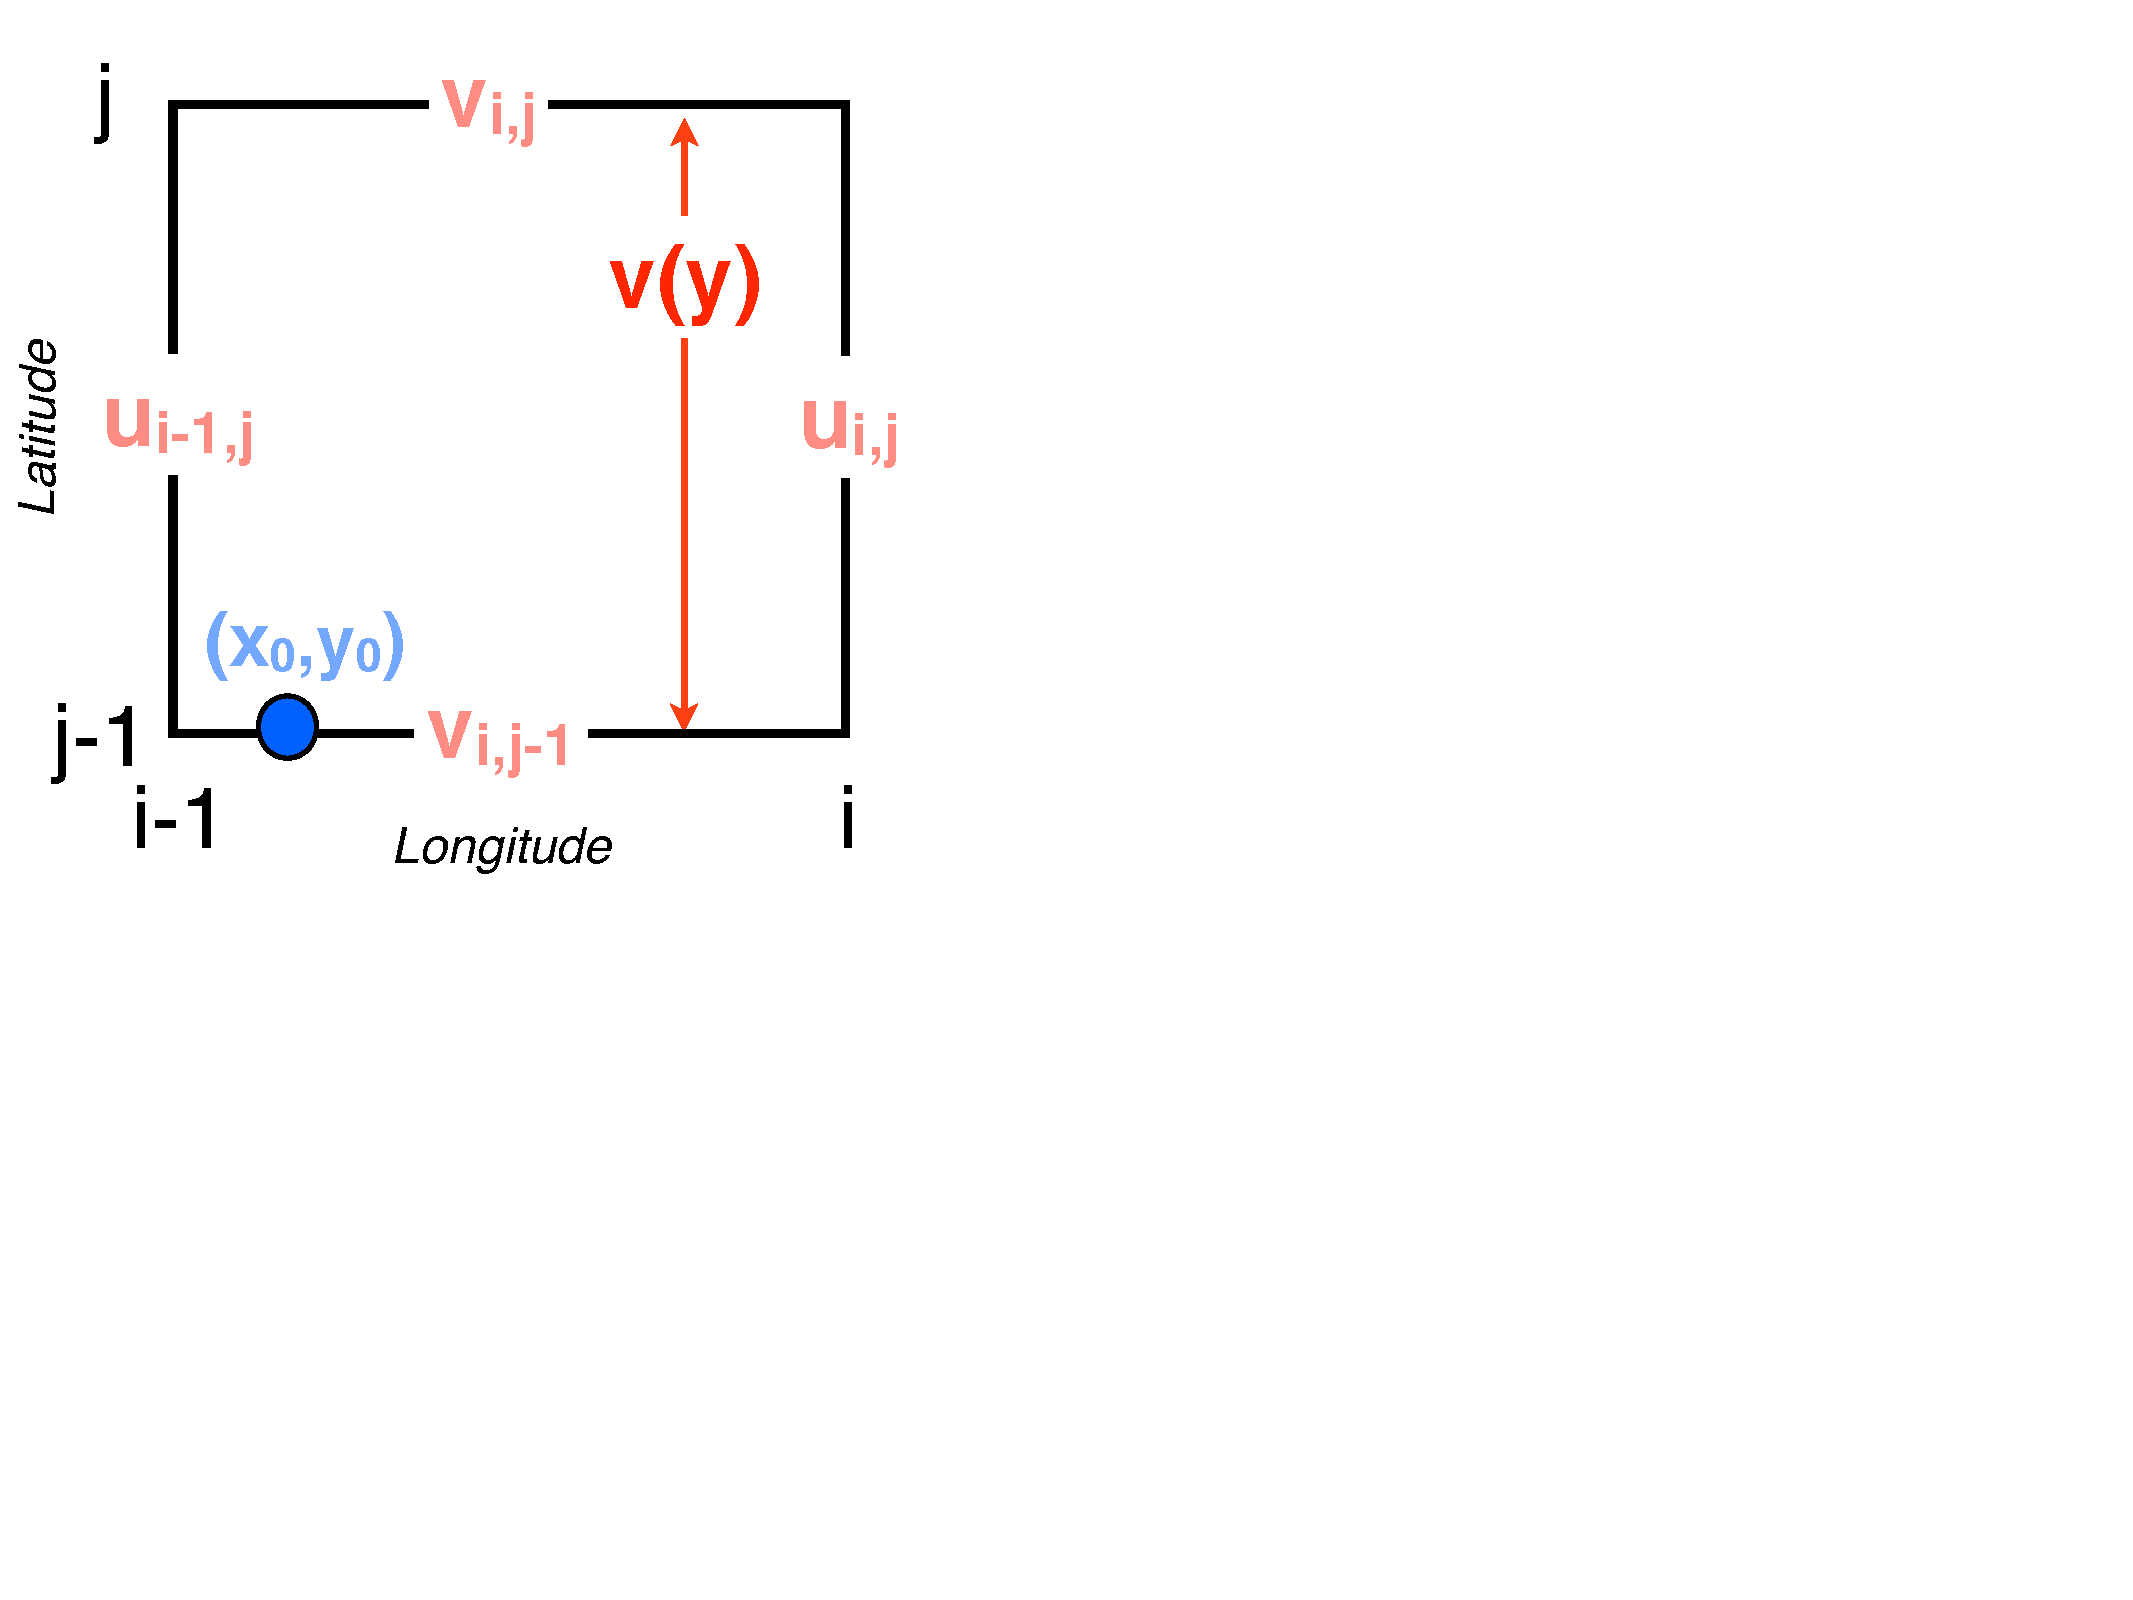
\includegraphics[width=.5\textwidth]{figures/tracmass_box6}
	\end{figure}
	{\Large Same process in $y$ and $z$ directions}
	\tiny{\\After TRACMASS documentation. http://www.tracmass.org, http://doos.misu.su.se/tracmass/}
\end{frame}
\begin{frame}[t,noframenumbering]\frametitle{Lagrangian Trajectory Model}
	\begin{figure}[htbp]
		\centering
		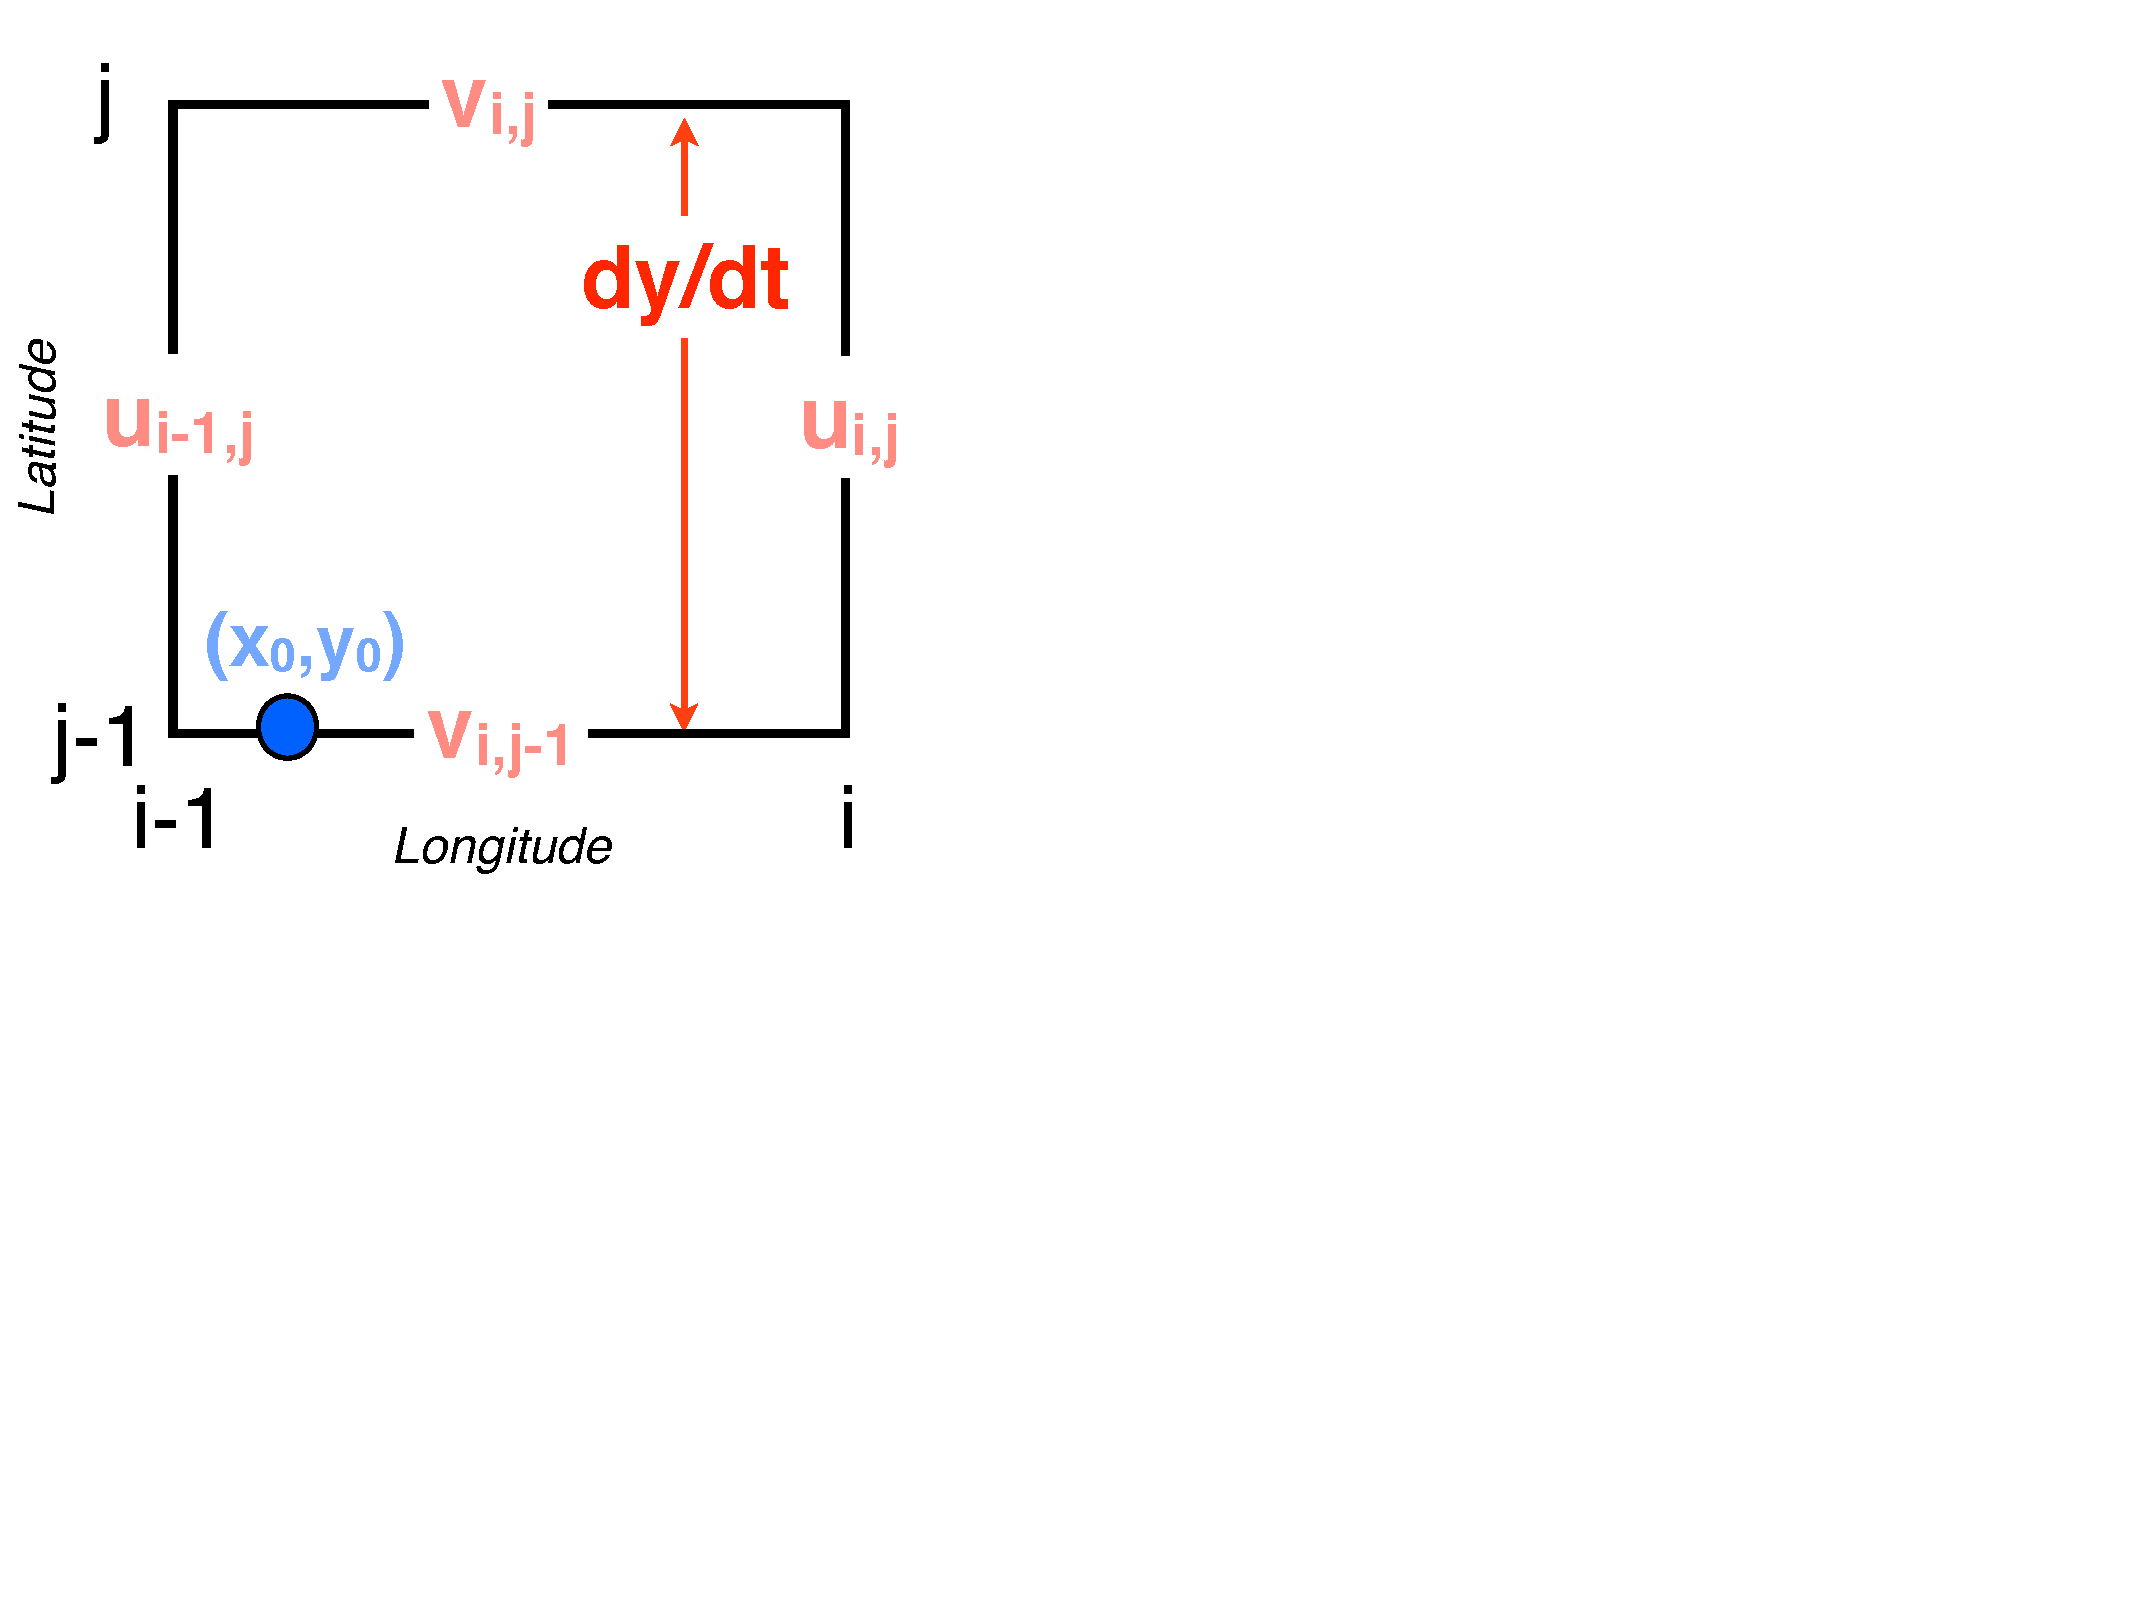
\includegraphics[width=.5\textwidth]{figures/tracmass_box7}
	\end{figure}
	{\Large Same process in $y$ and $z$ directions}
	\tiny{\\After TRACMASS documentation. http://www.tracmass.org, http://doos.misu.su.se/tracmass/}
\end{frame}
\begin{frame}[t,noframenumbering]\frametitle{Lagrangian Trajectory Model}
	\begin{figure}[htbp]
		\centering
		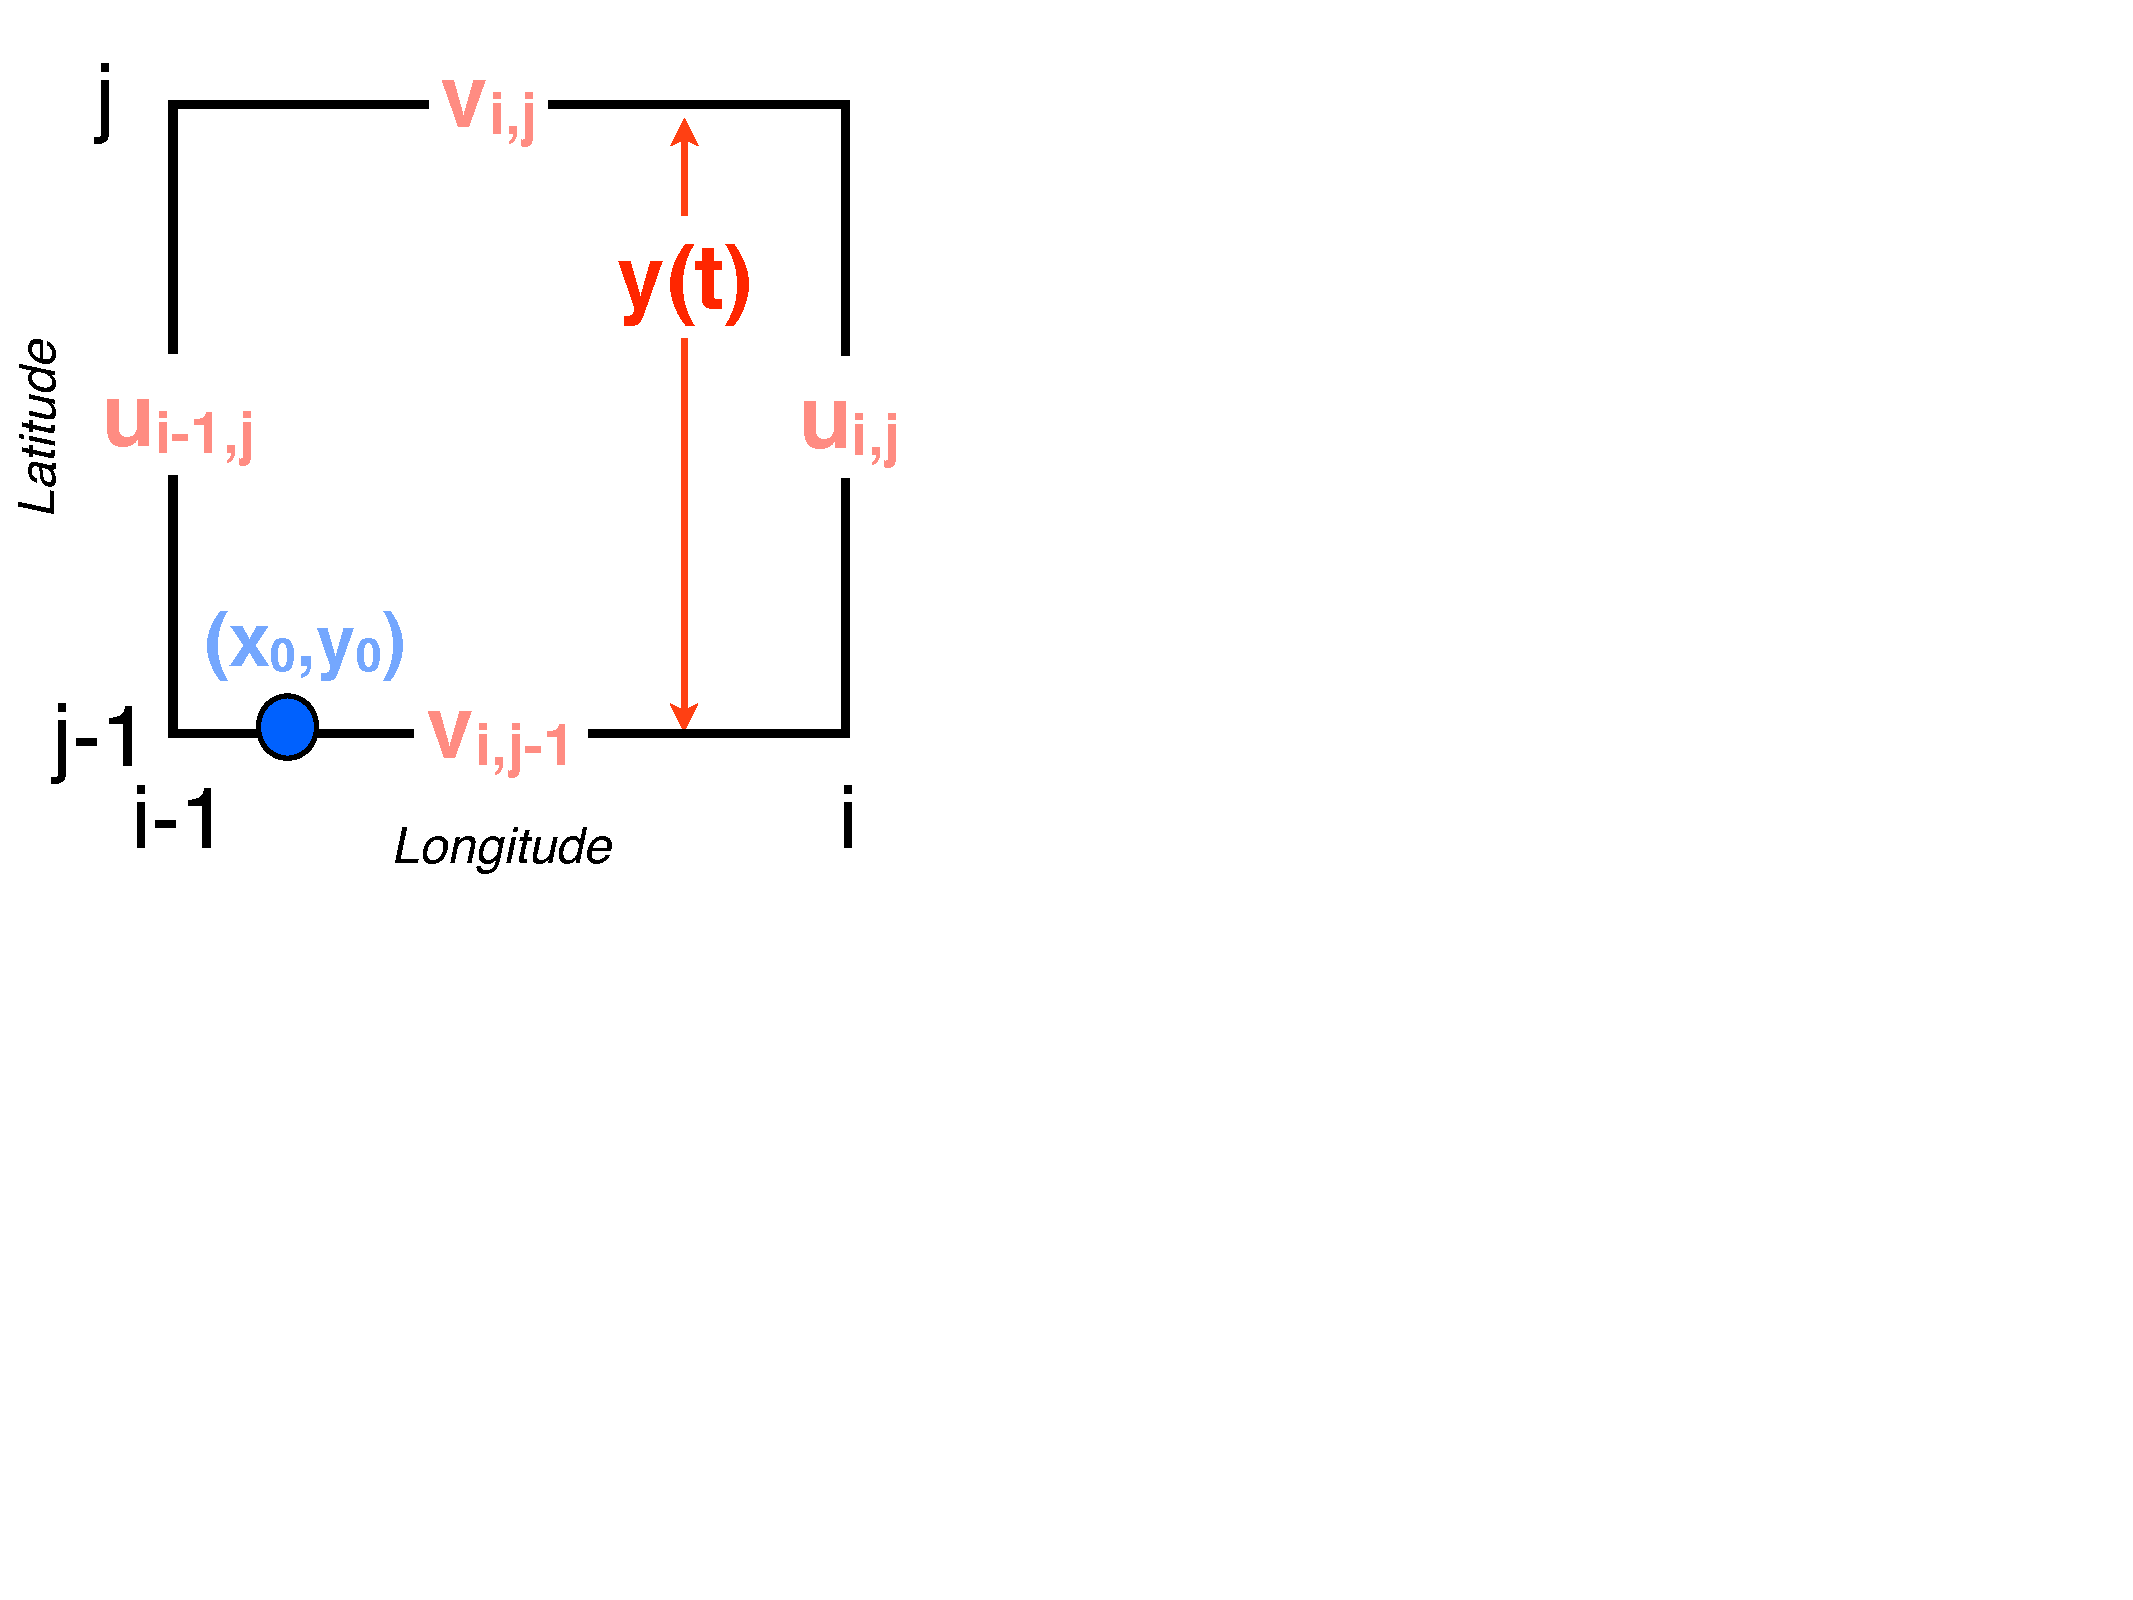
\includegraphics[width=.5\textwidth]{figures/tracmass_box8}
	\end{figure}
	{\Large Same process in $y$ and $z$ directions}
	\tiny{\\After TRACMASS documentation. http://www.tracmass.org, http://doos.misu.su.se/tracmass/}
\end{frame}
\begin{frame}[t,noframenumbering]\frametitle{Lagrangian Trajectory Model}
	\begin{figure}[htbp]
		\centering
		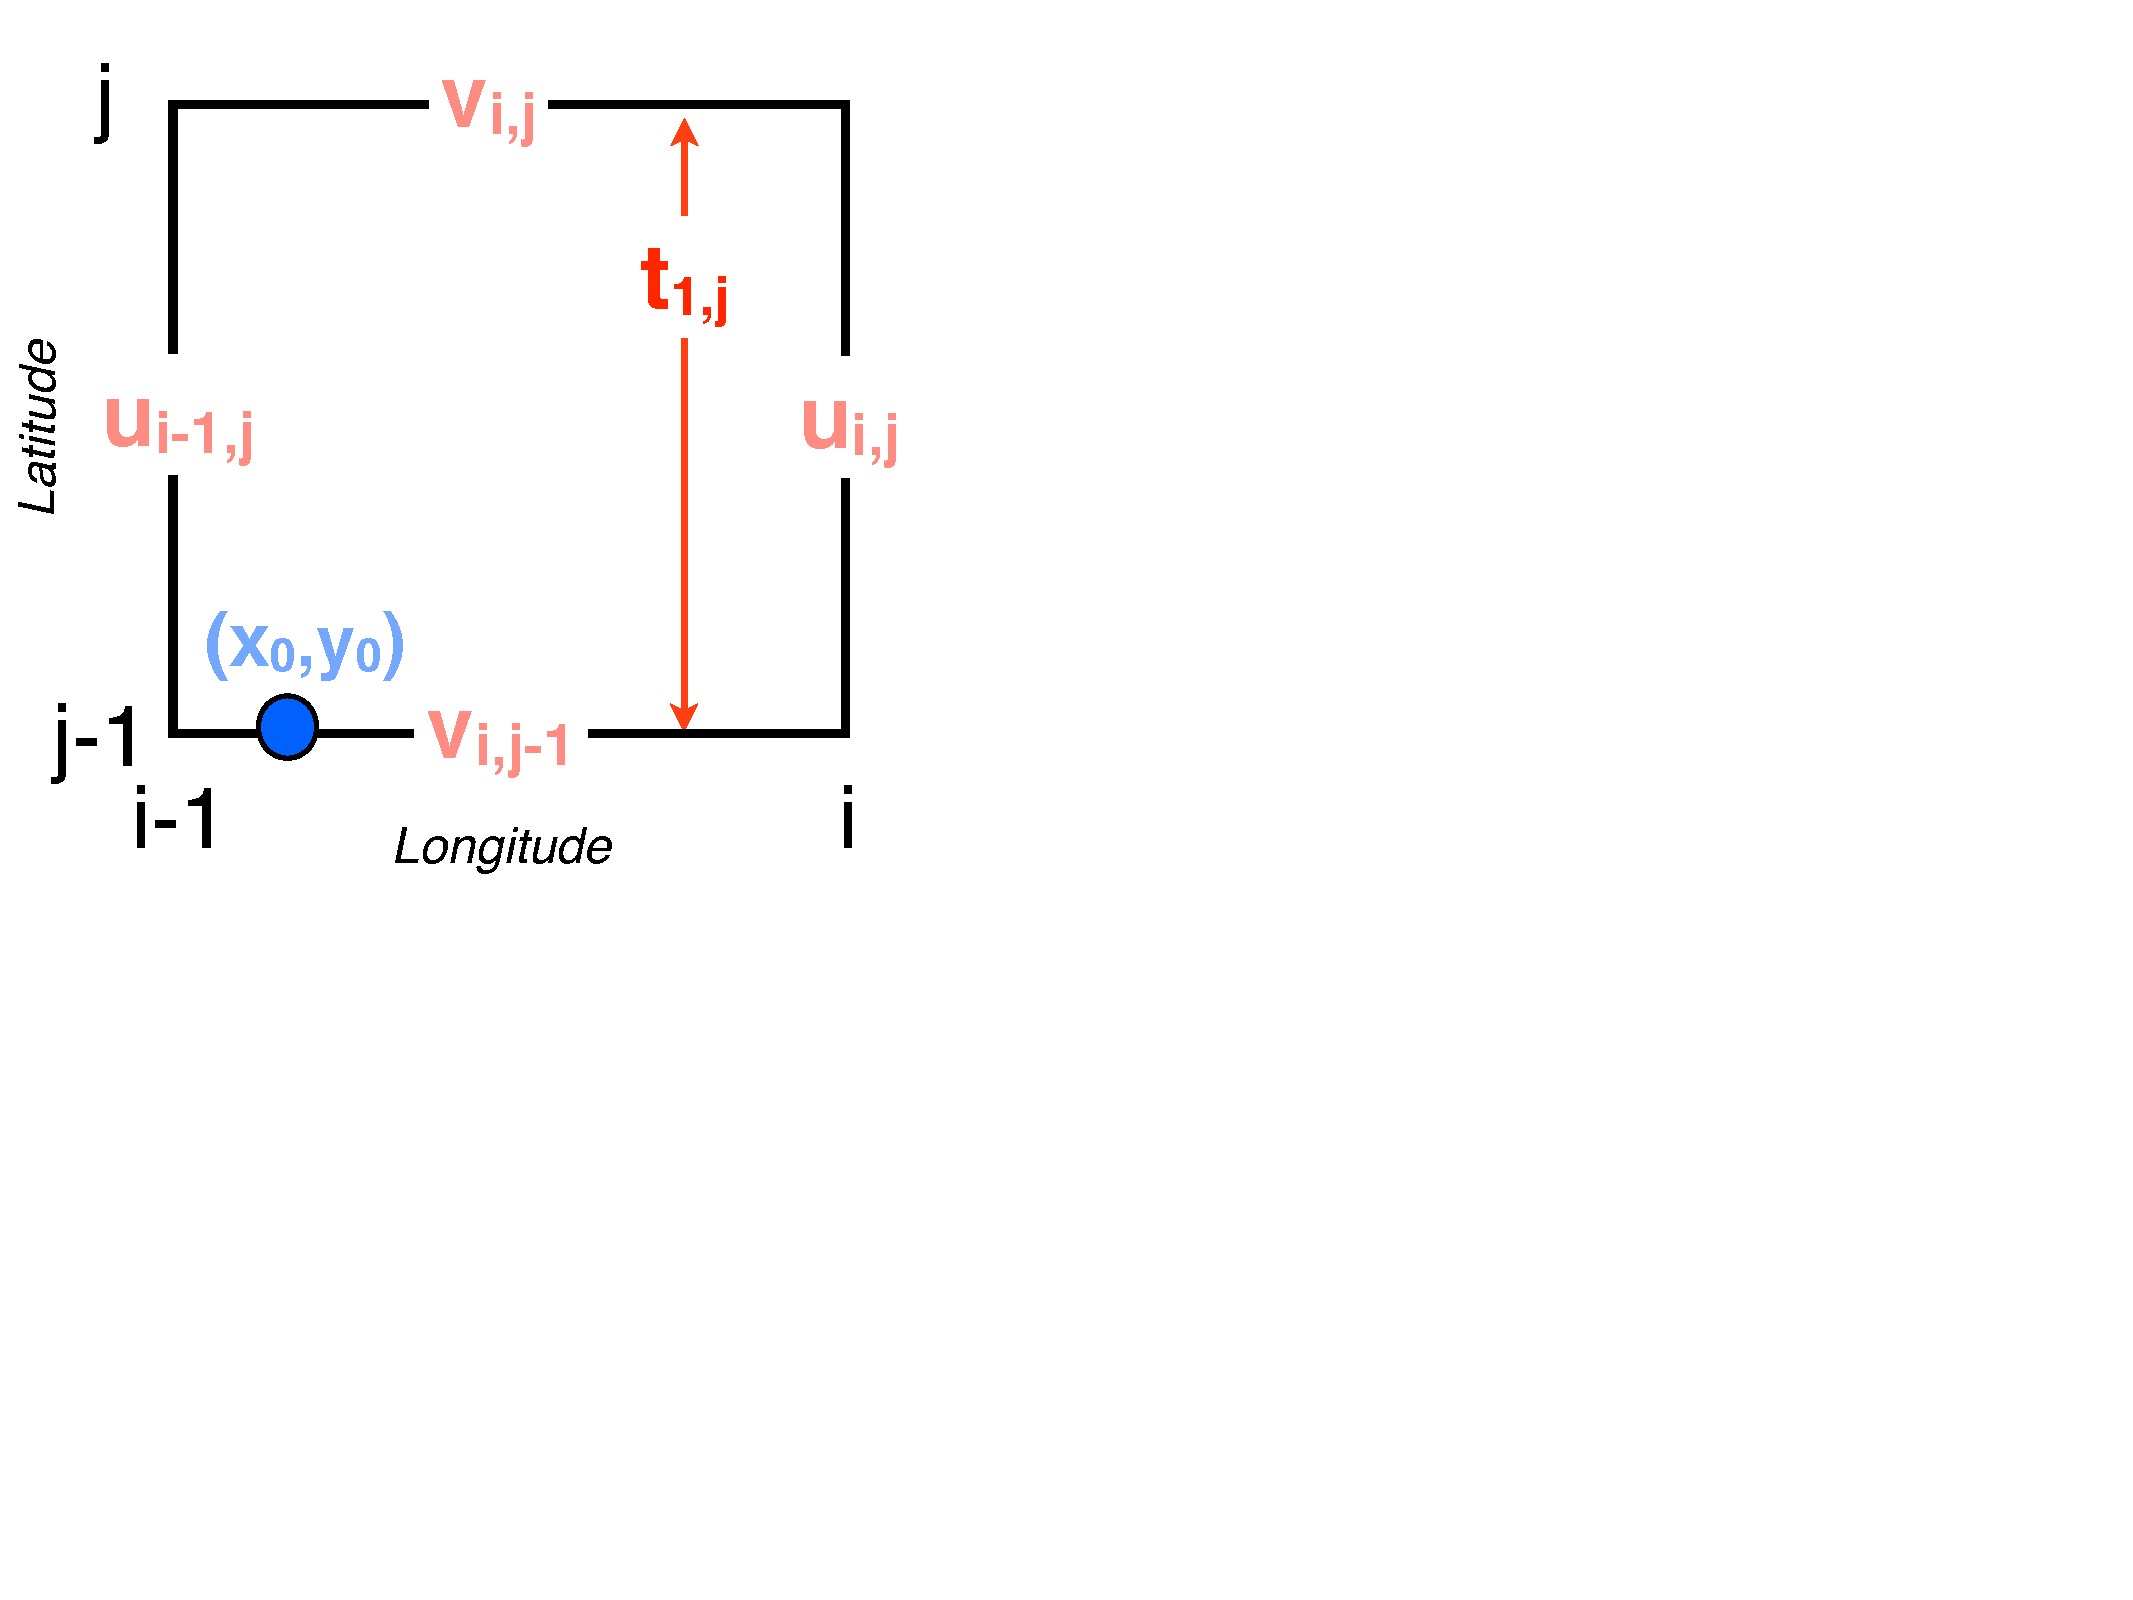
\includegraphics[width=.5\textwidth]{figures/tracmass_box9}
	\end{figure}
	{\Large Same process in $y$ and $z$ directions}
	\tiny{\\After TRACMASS documentation. http://www.tracmass.org, http://doos.misu.su.se/tracmass/}
\end{frame}
\begin{frame}[t,noframenumbering]\frametitle{Lagrangian Trajectory Model}
	\begin{figure}[htbp]
		\centering
		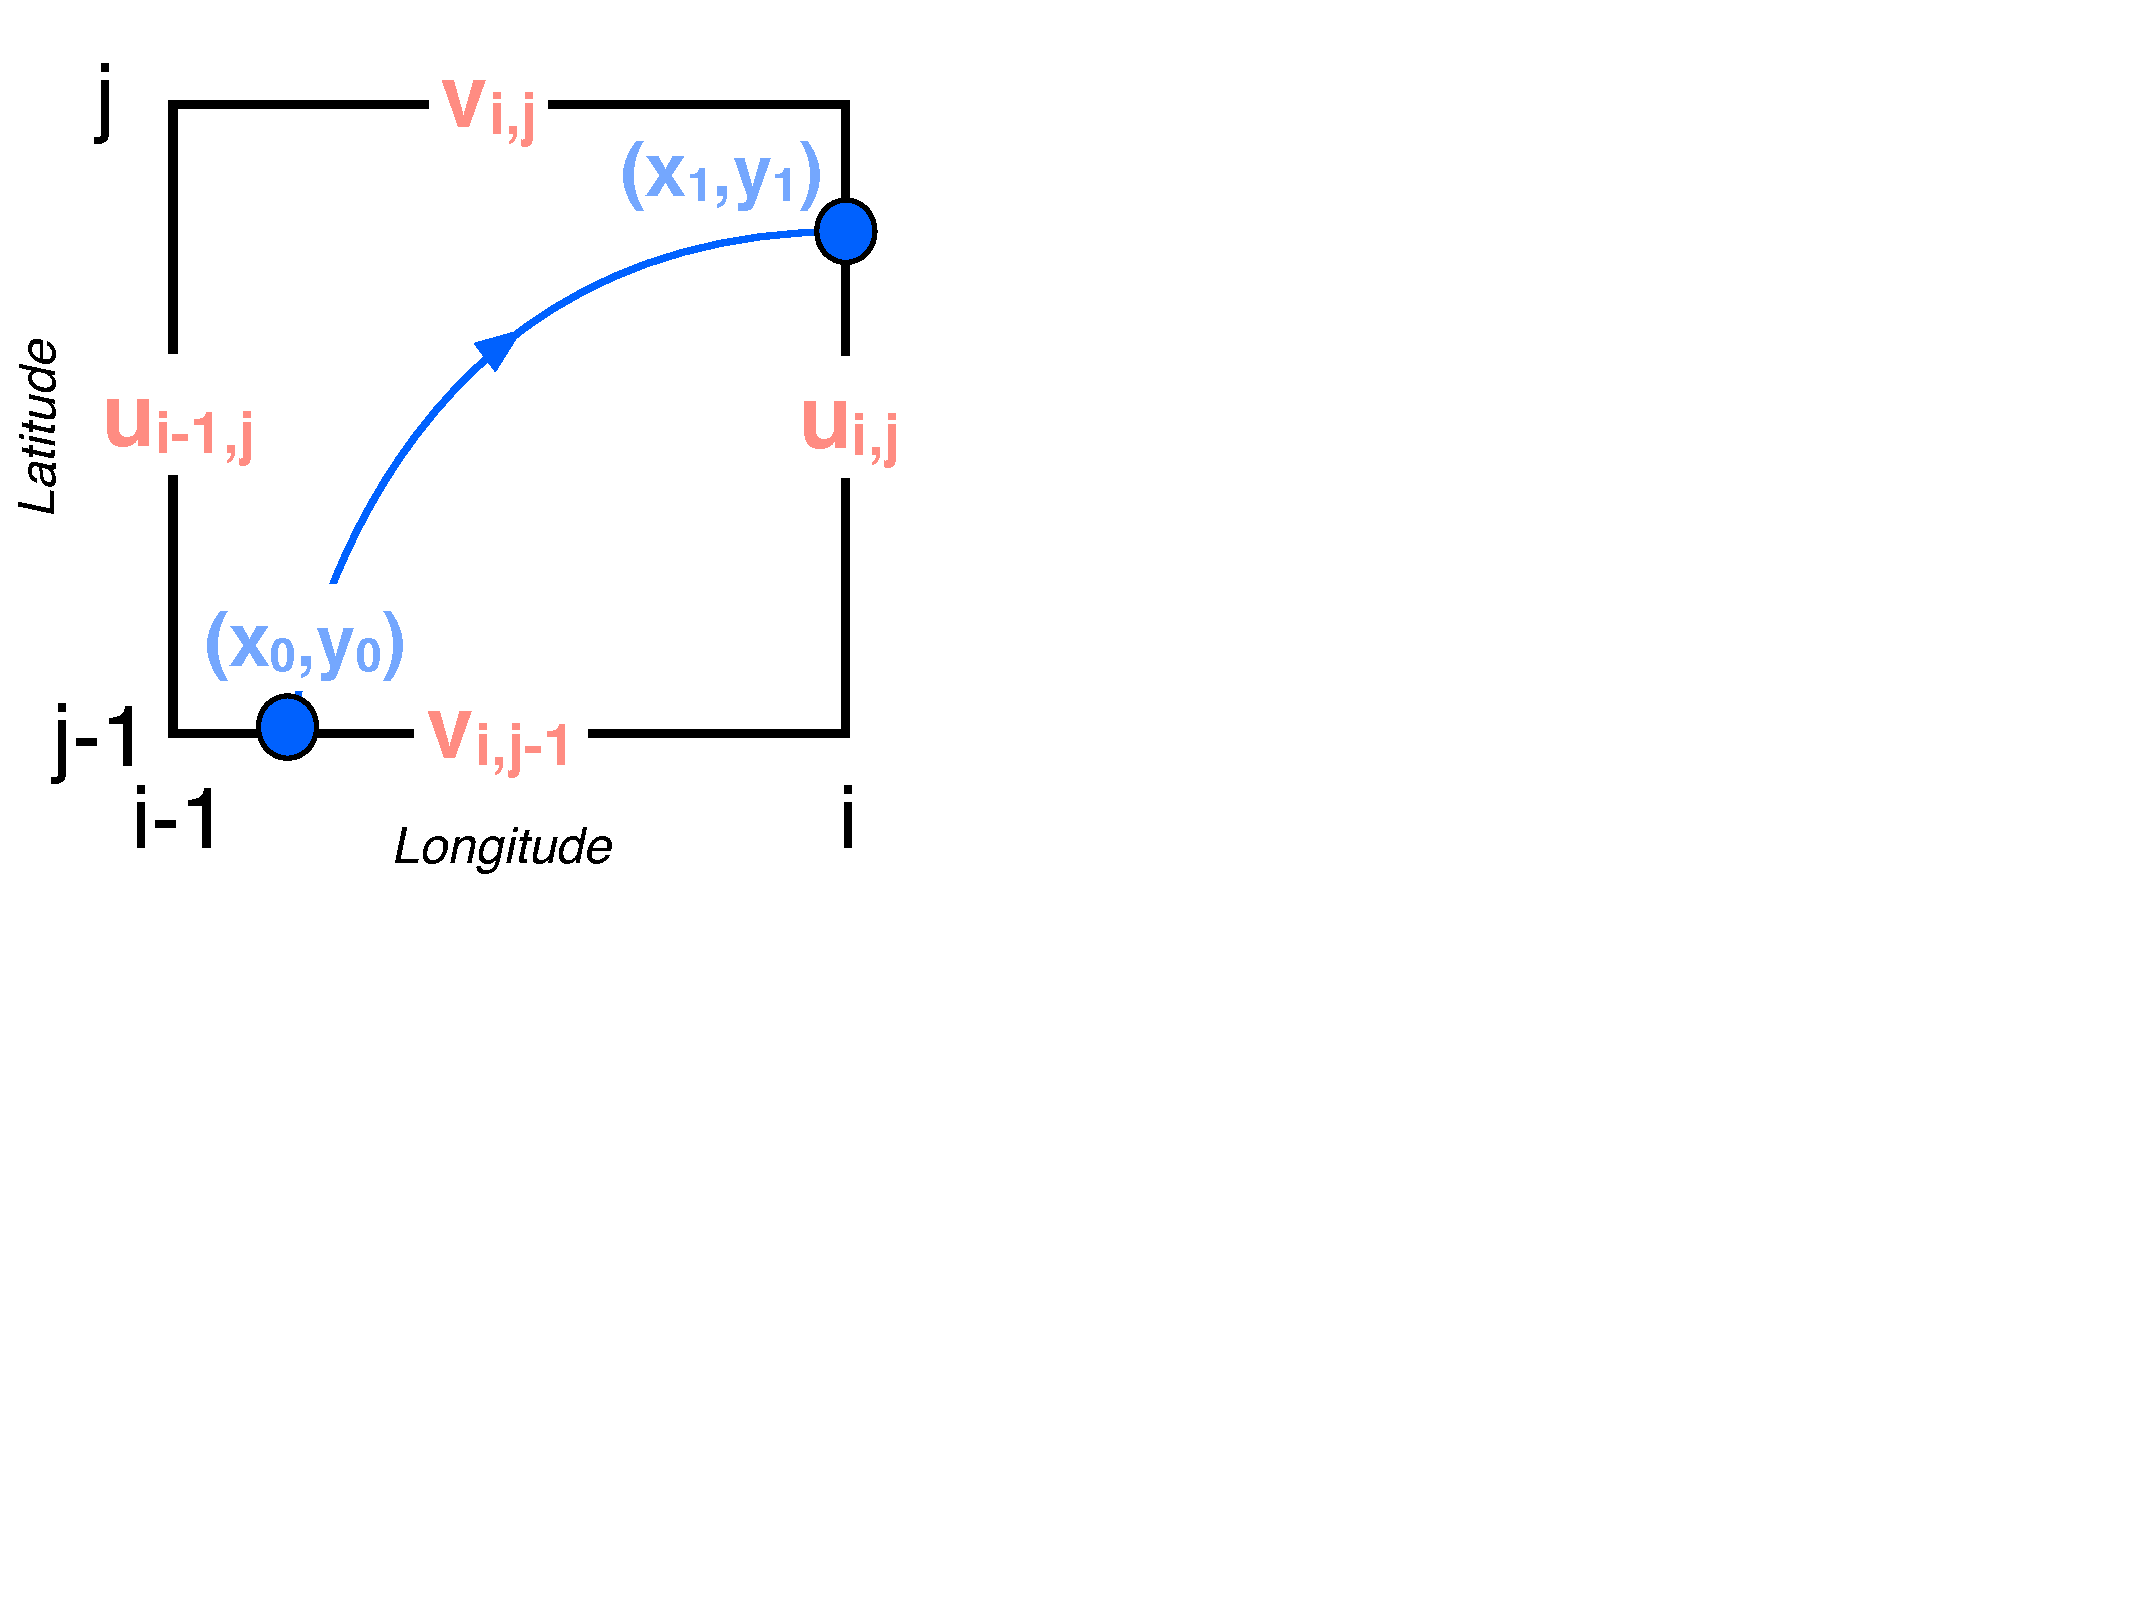
\includegraphics[width=.5\textwidth]{figures/tracmass_box10}
	\end{figure}
	{\Large Minimum overall time is used to calculate position}
	\tiny{\\After TRACMASS documentation. http://www.tracmass.org, http://doos.misu.su.se/tracmass/}
\end{frame}
\begin{frame}[t,noframenumbering]\frametitle{Lagrangian Trajectory Model}
	\begin{figure}[htbp]
		\centering
		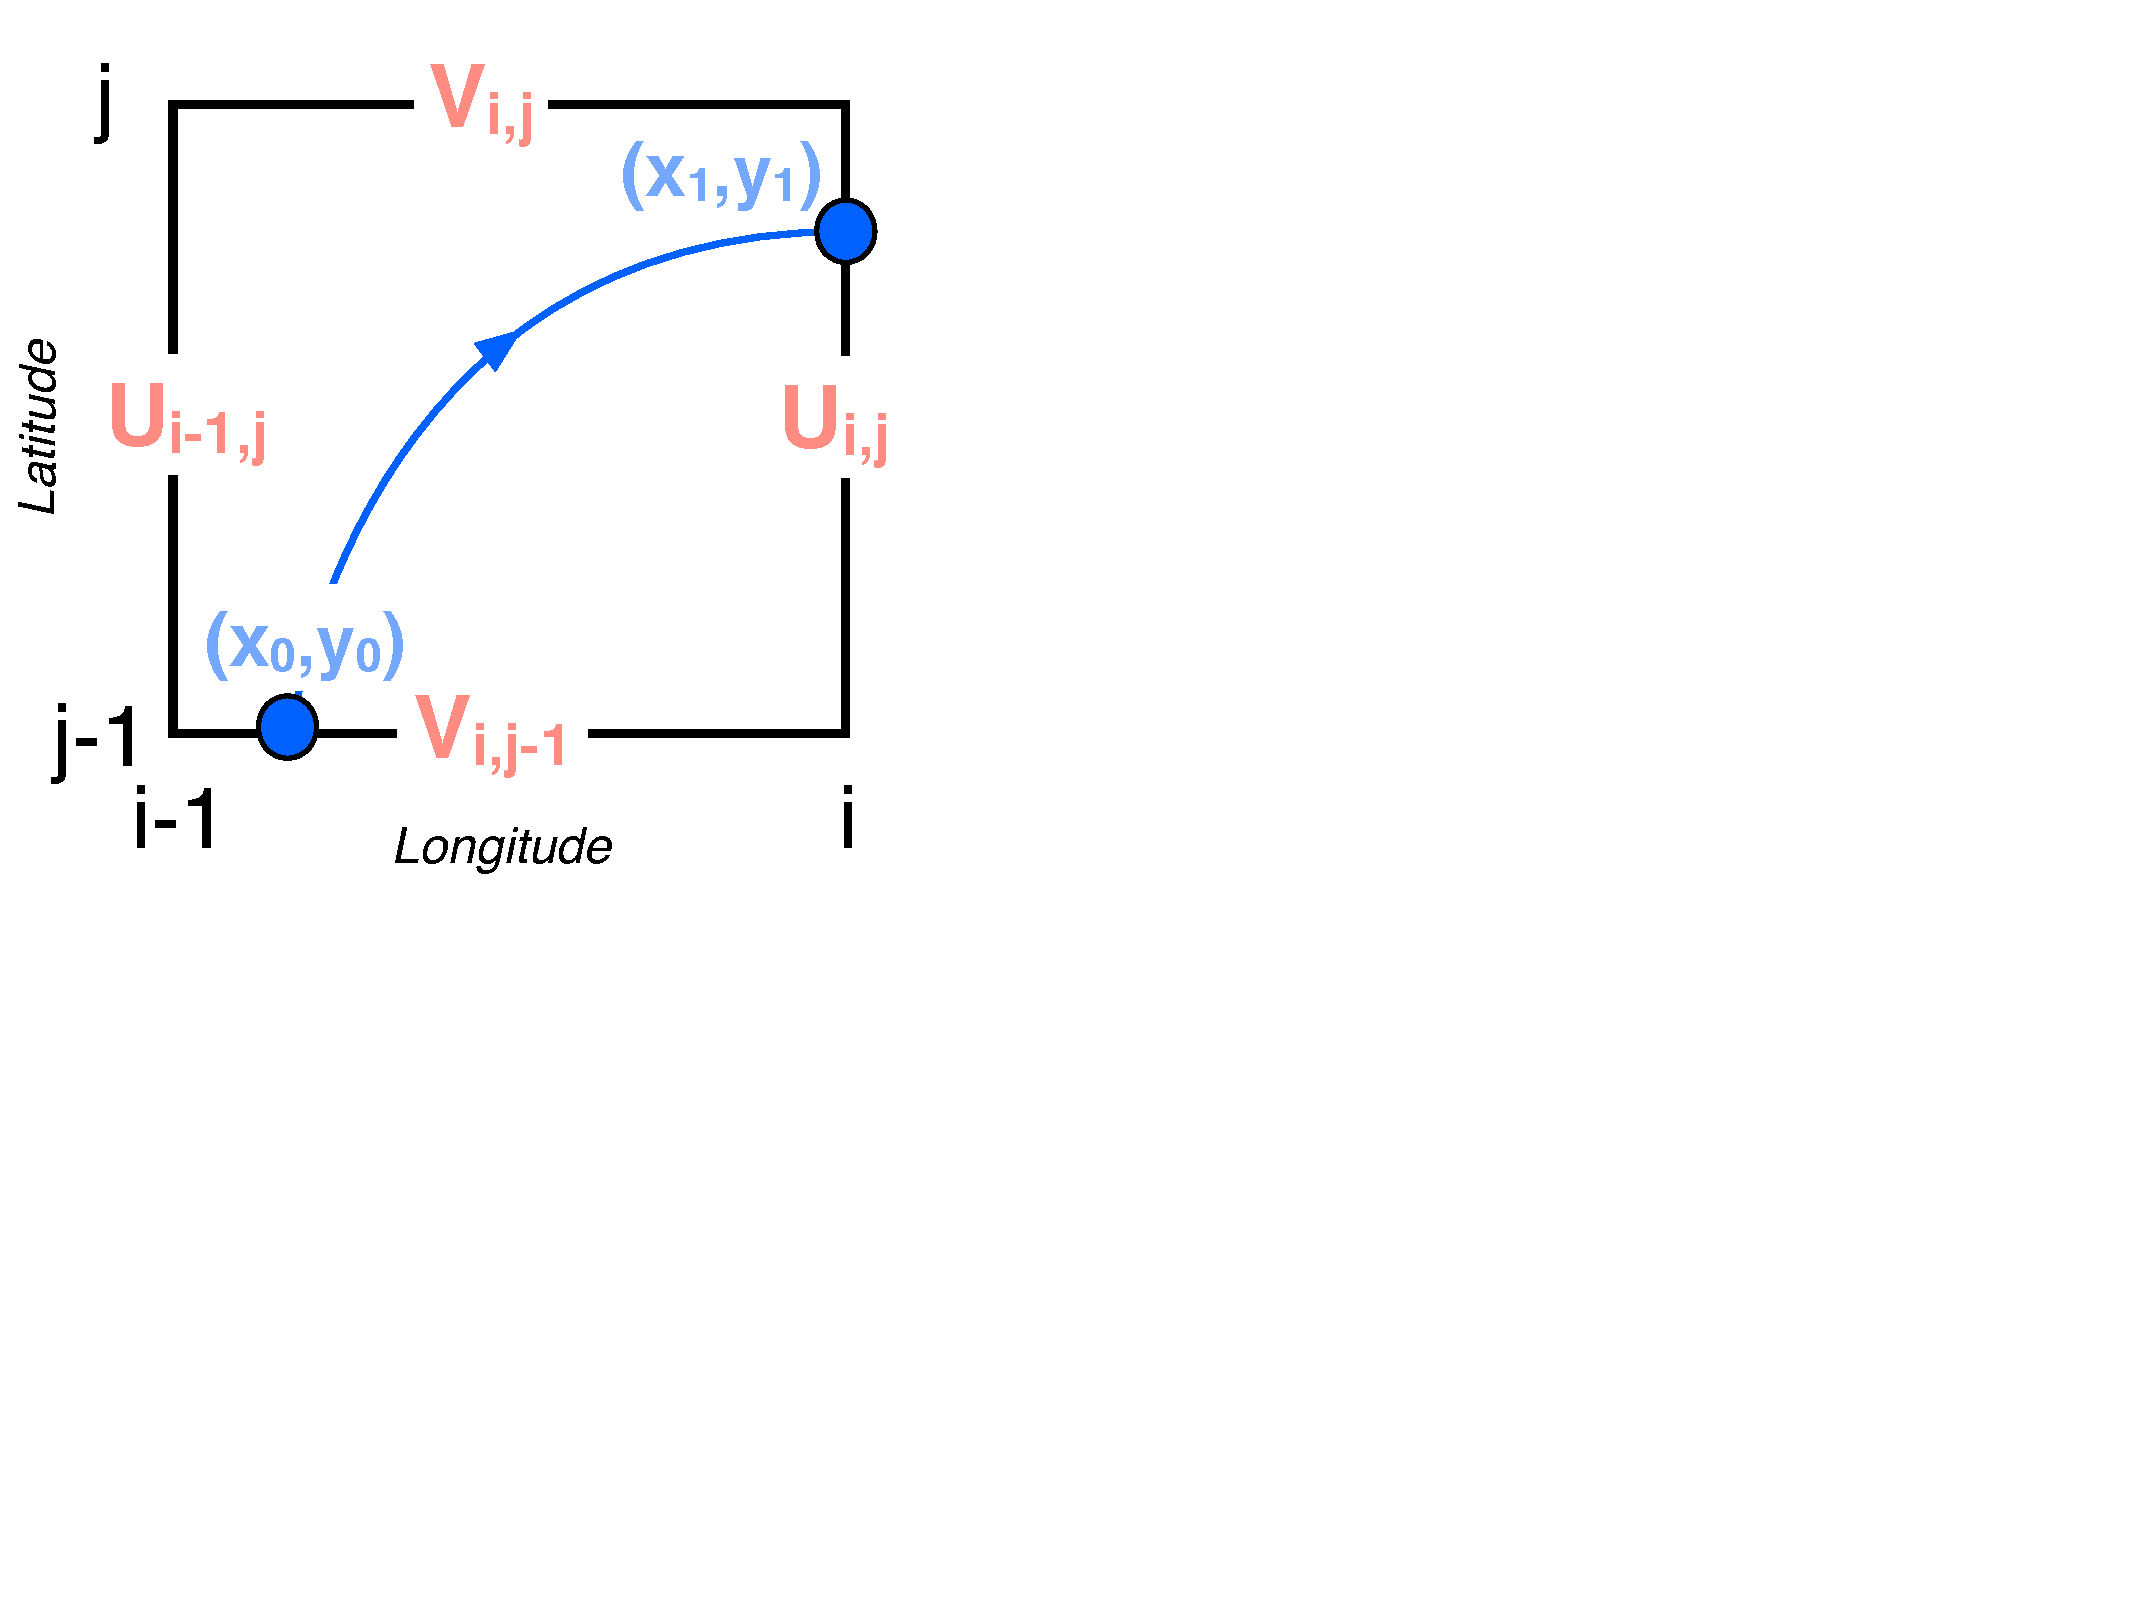
\includegraphics[width=.5\textwidth]{figures/tracmass_box11}
	\end{figure}
	{\Large Instead of velocities, use fluxes to allow for differences in grid sizing}
	\tiny{\\After TRACMASS documentation. http://www.tracmass.org, http://doos.misu.su.se/tracmass/}
\end{frame}

\begin{frame}[t]\frametitle{TRACMASS validation}
	\begin{figure}[htbp]
		\centering
		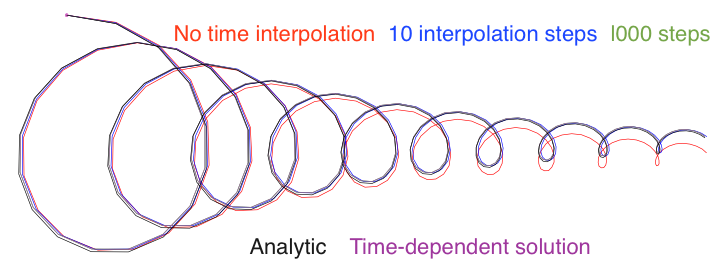
\includegraphics[width=\textwidth]{figures/validation}
	\end{figure}
	% \tiny{\\From WHERE}
\end{frame}

\begin{frame}[t]\frametitle{Drifter Trajectories}
% EXPLAIN SIMULATION DETAILS FOR DRIFTERS
	\begin{figure}
	  	\centering
	   	\includemovie[autoplay, poster, autopause, autoresume, controls, repeat
	   	]{\textheight}{0.8\textheight}{figures/drifter_movie.mp4}
		%\vskip-1ex
	\end{figure}
\end{frame}


%%% TracPy

\section{Wrapper}

\begin{frame}[t]\frametitle{TracPy}
    % SHOW DIAGRAM OF TRACPY VS. TRACMASS, including tracpy class and parts
    \vskip-2ex
	\begin{figure}[htbp]
		\centering
		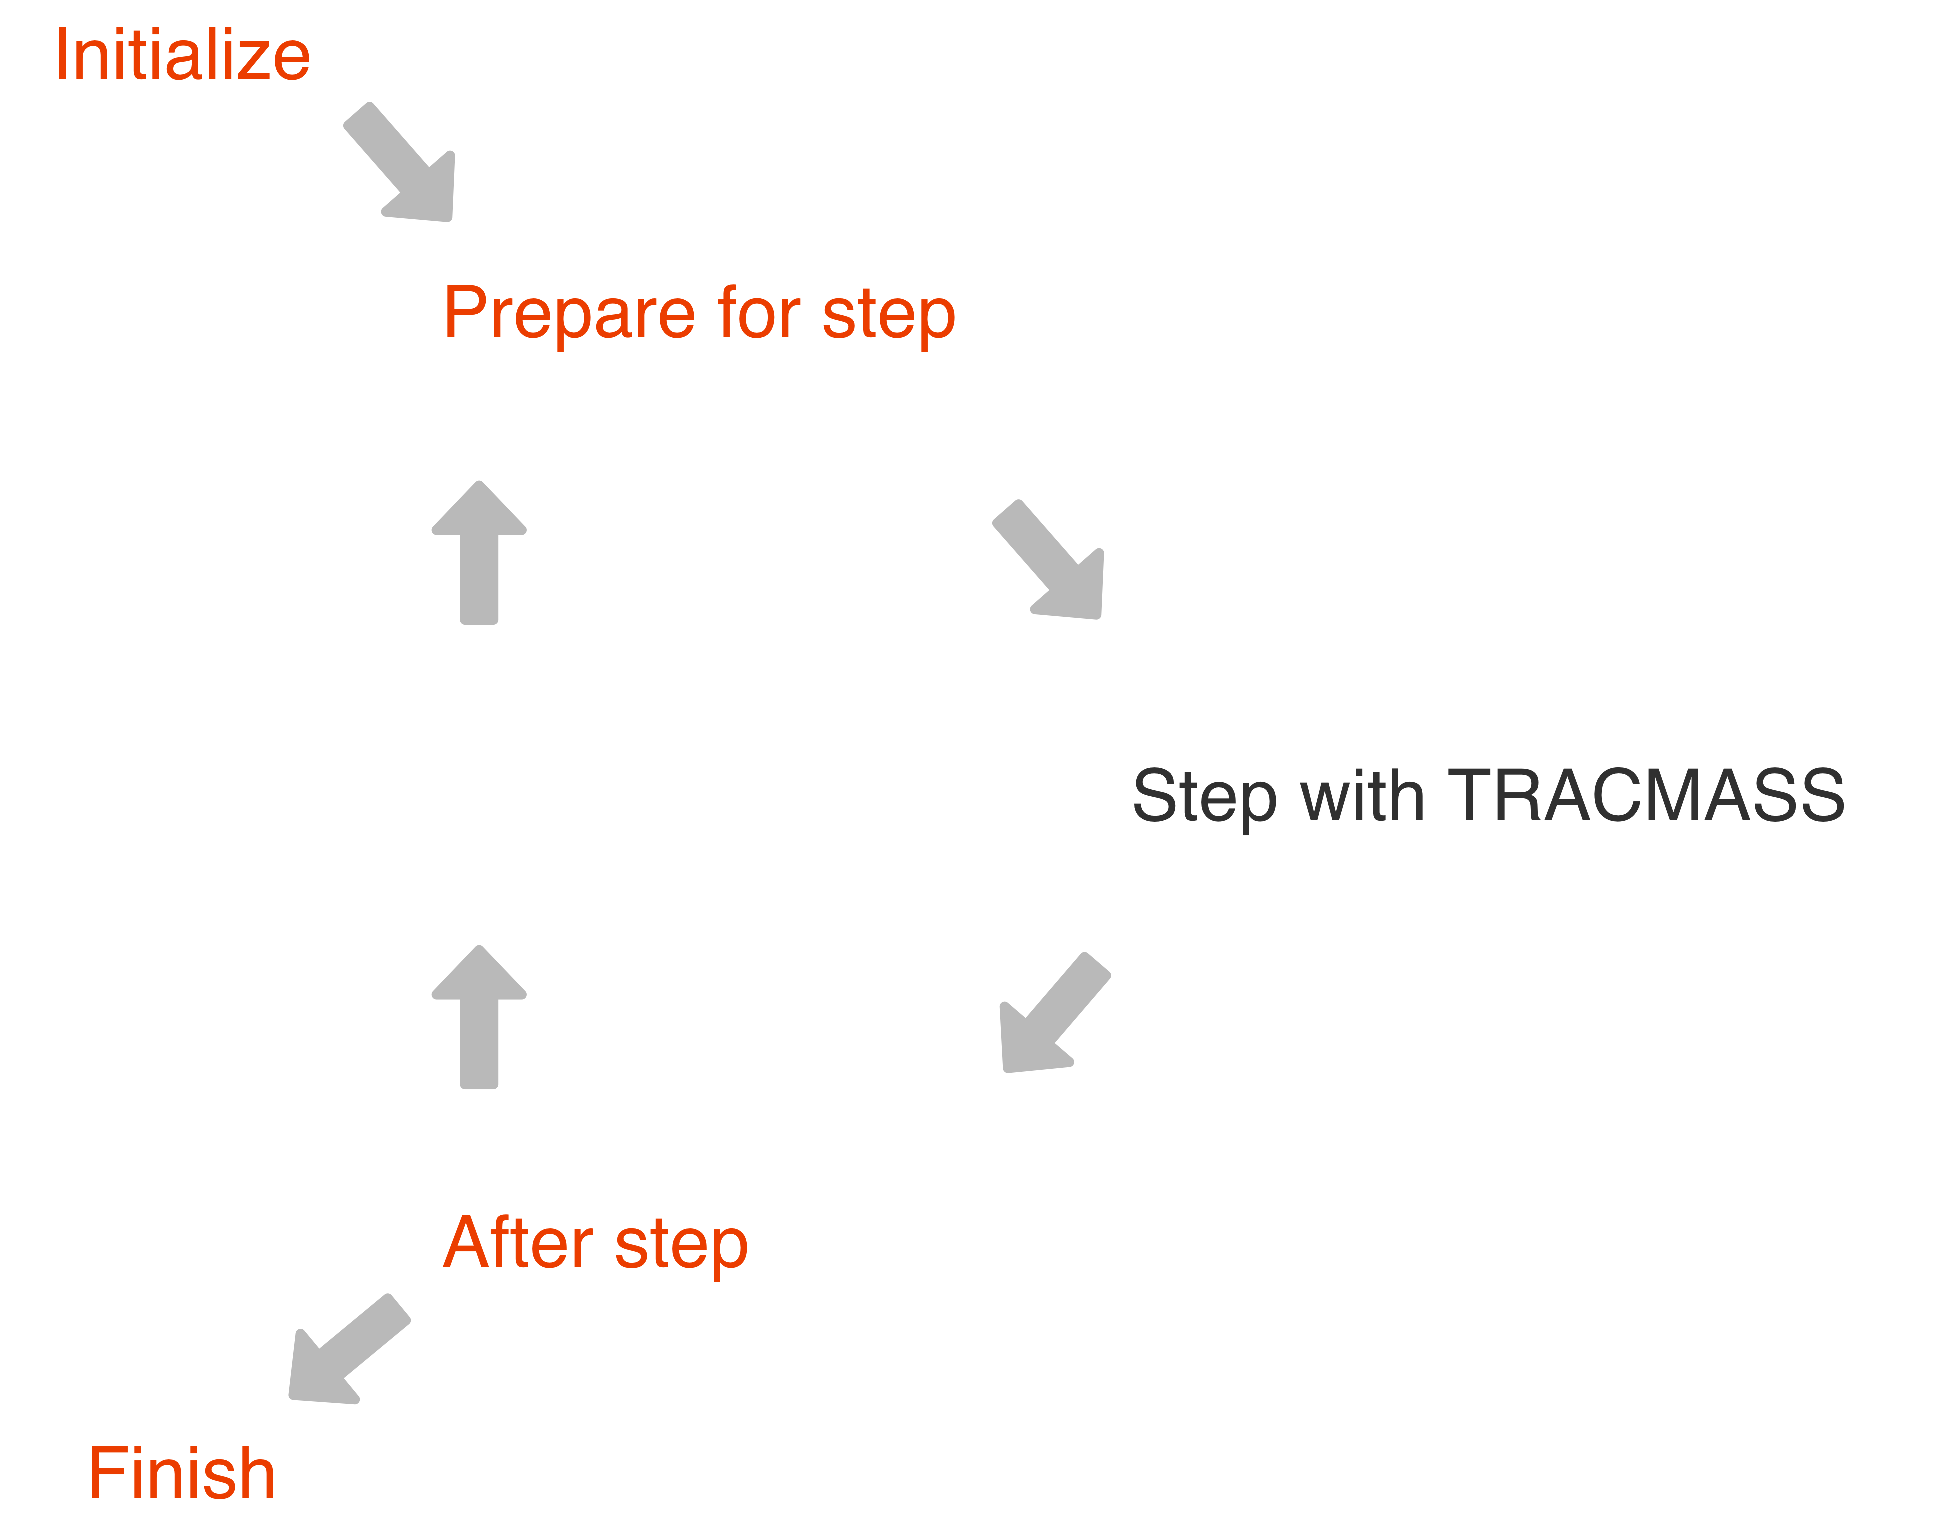
\includegraphics[width=0.8\textwidth]{figures/tracpy-tracmass}
	\end{figure}
\end{frame}

\begin{frame}[t]\frametitle{TracPy performance}
    \vskip4ex
	\begin{figure}[htbp]
		\centering
		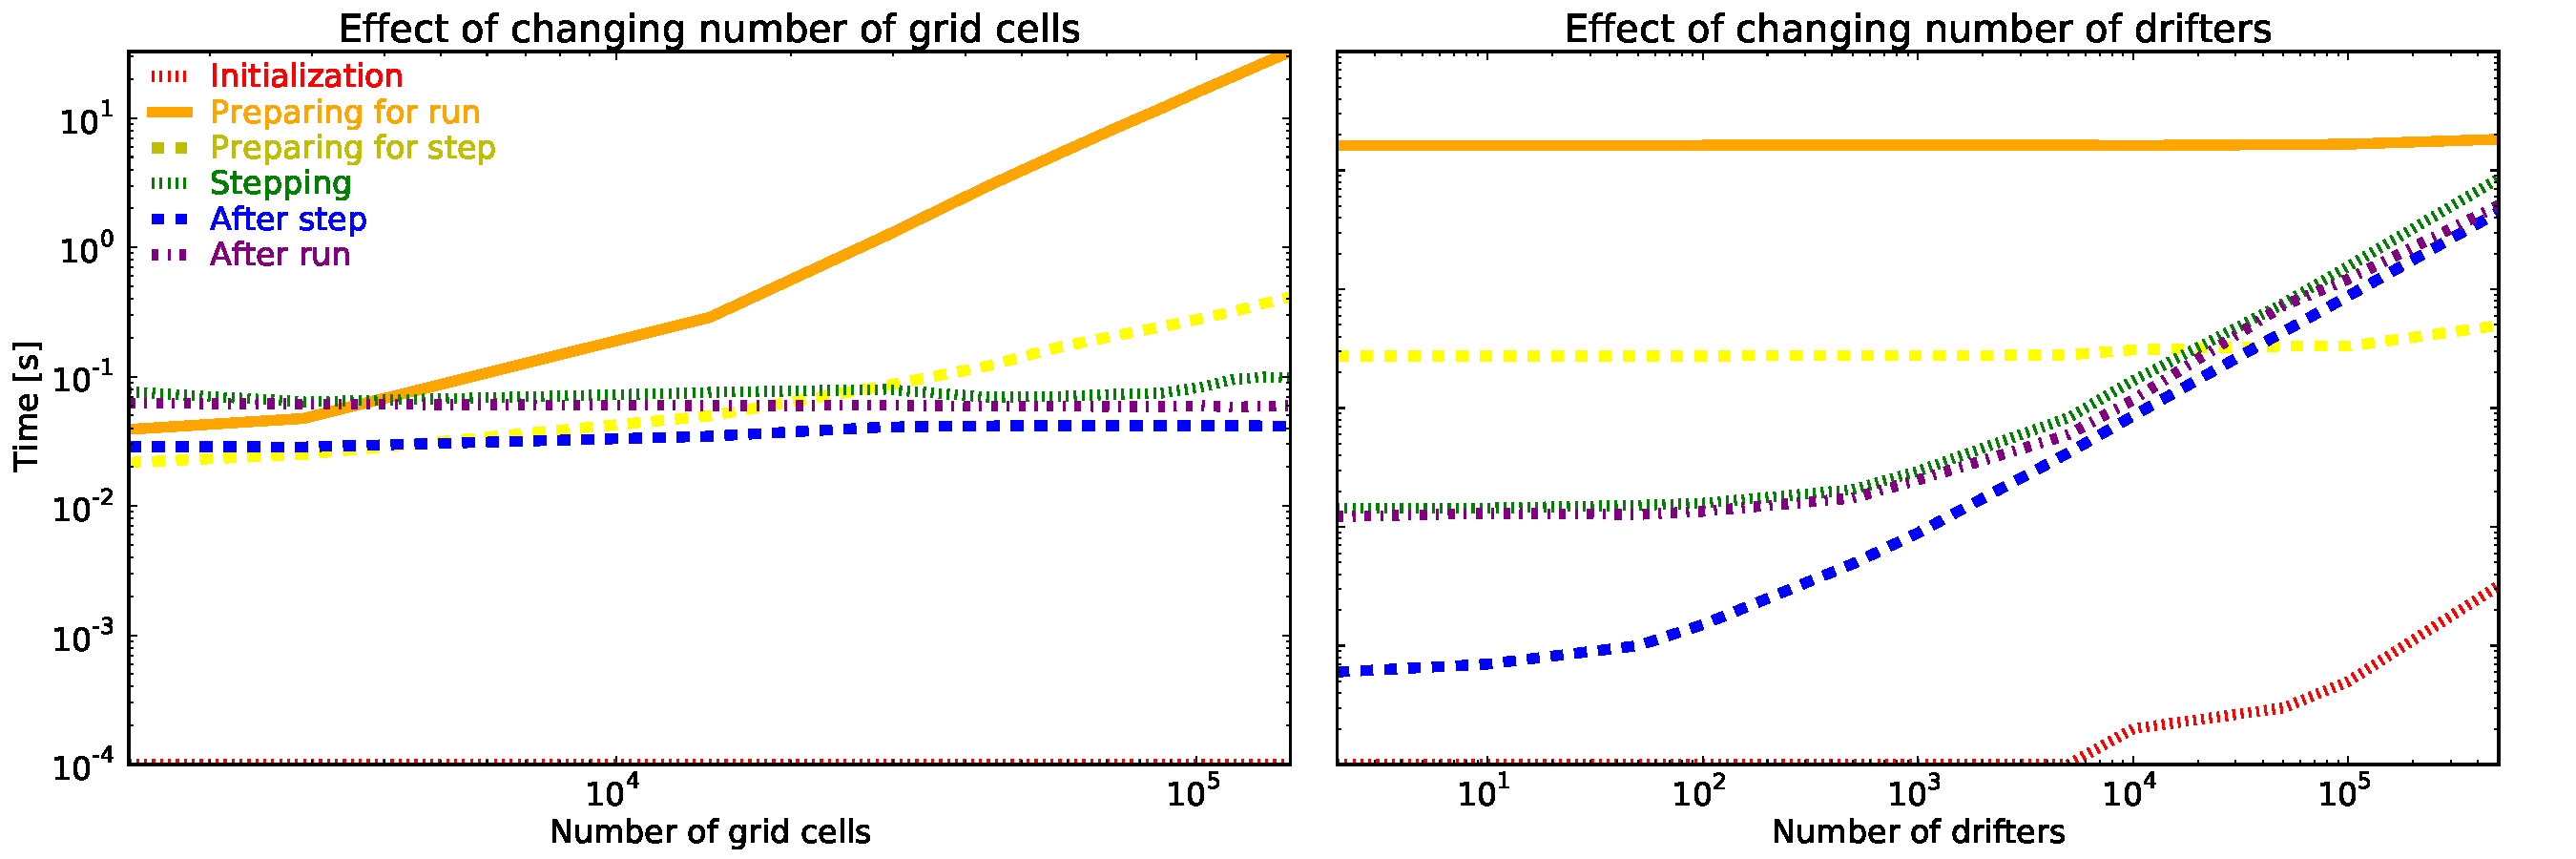
\includegraphics[width=\textwidth]{figures/comparison}
	\end{figure}
\end{frame}

\begin{frame}[t]\frametitle{netCDF performance}
\vskip4ex
\begin{table}
\begin{tabular}{llll}
  & netCDF3  & netCDF4C & \% decrease \\
Simulation run time (s) & 1038 & 1038 & 0 \\
File save time (s) & 3527 & 131 & 96 \\
File size (GB) & 3.6 & 2.1 & 42 
\end{tabular}
\end{table}
\end{frame}


\begin{frame}[t]\frametitle{Parallelization}
	\begin{figure}[htbp]
		\centering
		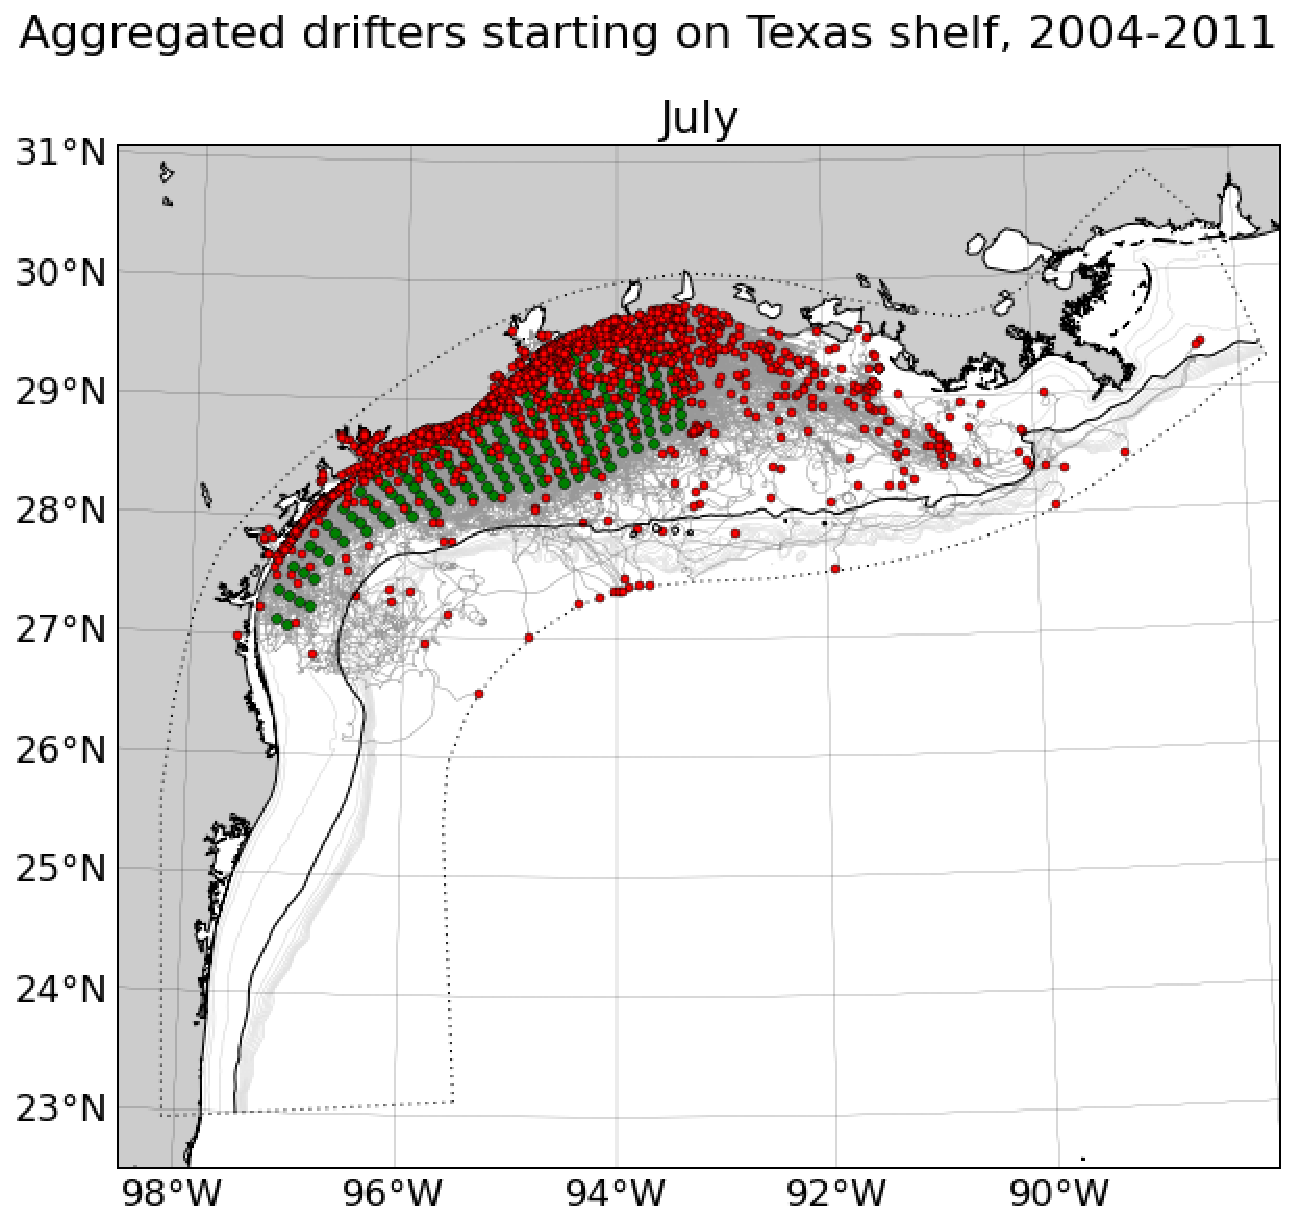
\includegraphics[width=0.6\textwidth]{figures/area3_tracks}
		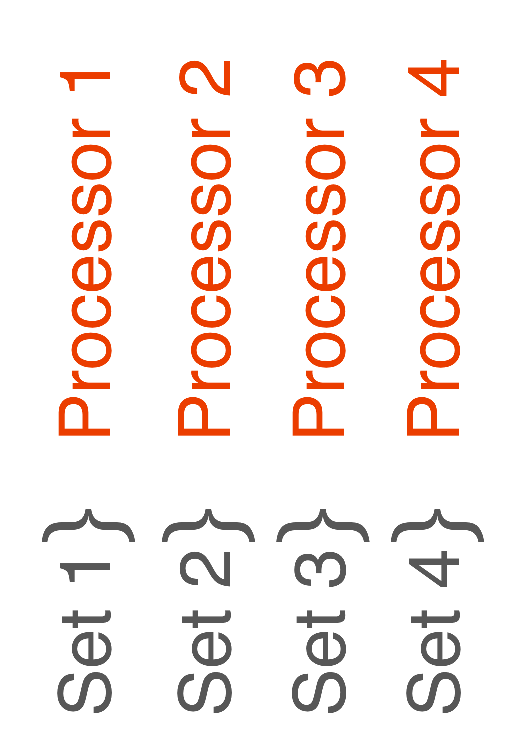
\includegraphics[width=0.27\textwidth]{figures/parallelization}
	\end{figure}
\end{frame}

% \begin{frame}[t]\frametitle{Lessons learned}
    


% \end{frame}

\begin{frame}[t]\frametitle{Future work}
\begin{itemize}
	\item {\Large Integration into NOAA's GNOME oil tracking system}
	\item[] ~
	\item {\Large Improve grid read in speed and memory required}
	\item[] ~
	\item {\Large Append output to track file instead of storing for full run}
	\item[] ~
	\item {\Large Possibly rearrange drifter arrangement in output file to reduce nan storage}
	\item[] ~
	\item {\Large Storage could be updated to full netCDF4 format.}
	\item[] ~
	\item {\Large The modularity of the TracPy class should be improved.}
\end{itemize}
\end{frame}

%%% Uses

\section{Uses of TracPy}

\begin{frame}[t]\frametitle{Cross-shelf transport}
	\begin{figure}[htbp]
		\centering
		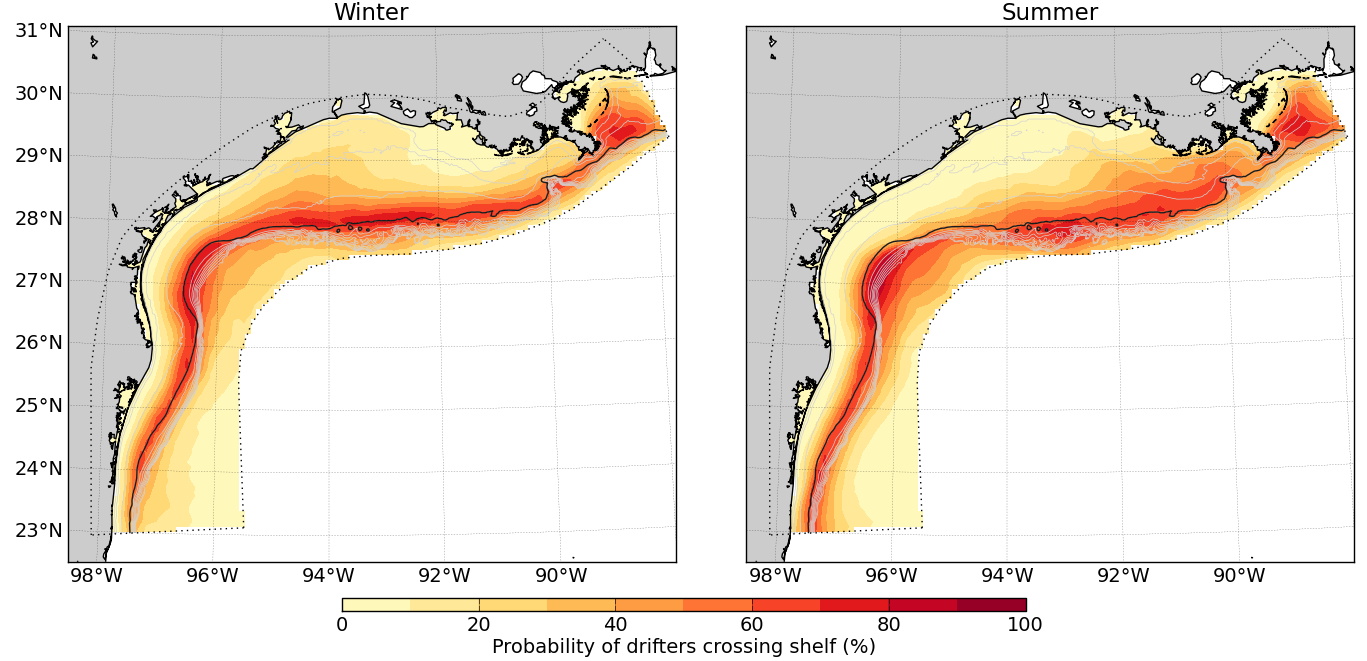
\includegraphics[width=\textwidth]{figures/seasonal100.png}
	\end{figure}
\end{frame}
\begin{frame}[t,noframenumbering]\frametitle{Cross-shelf transport}
	\begin{figure}[htbp]
		\centering
		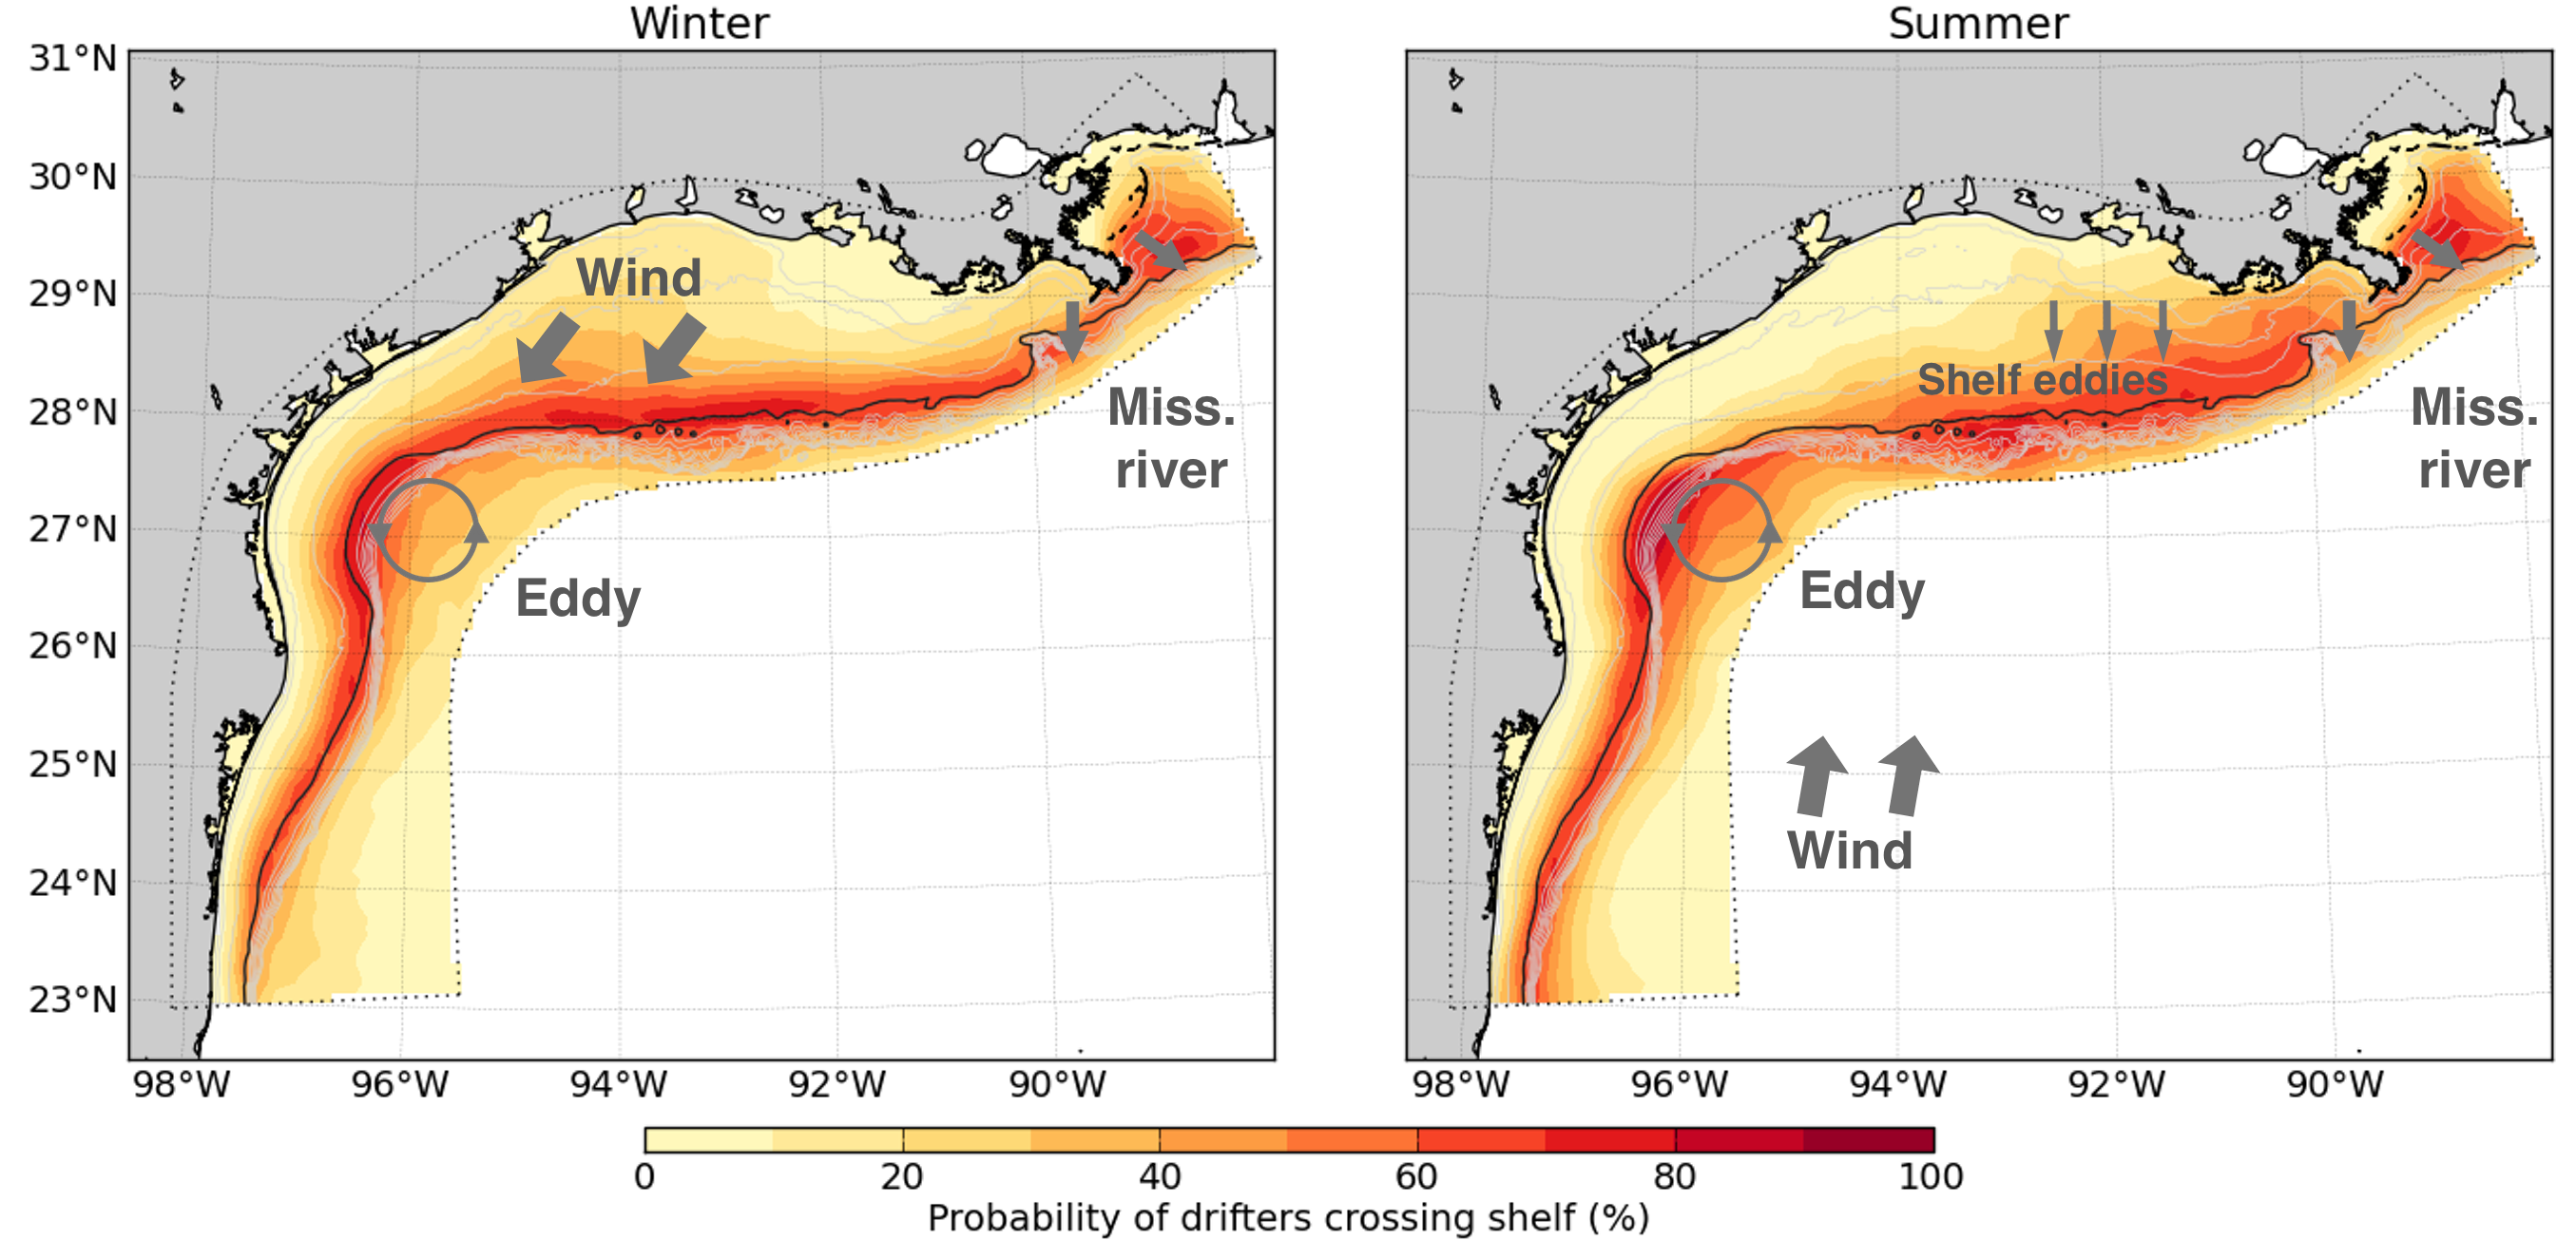
\includegraphics[width=\textwidth]{figures/seasonal100_allpictures.png}
	\end{figure}
\end{frame}

\begin{frame}[t]\frametitle{Coastline connectivity: Chenier Plain}
	\begin{figure}[htbp]
		\centering
		\only<1>{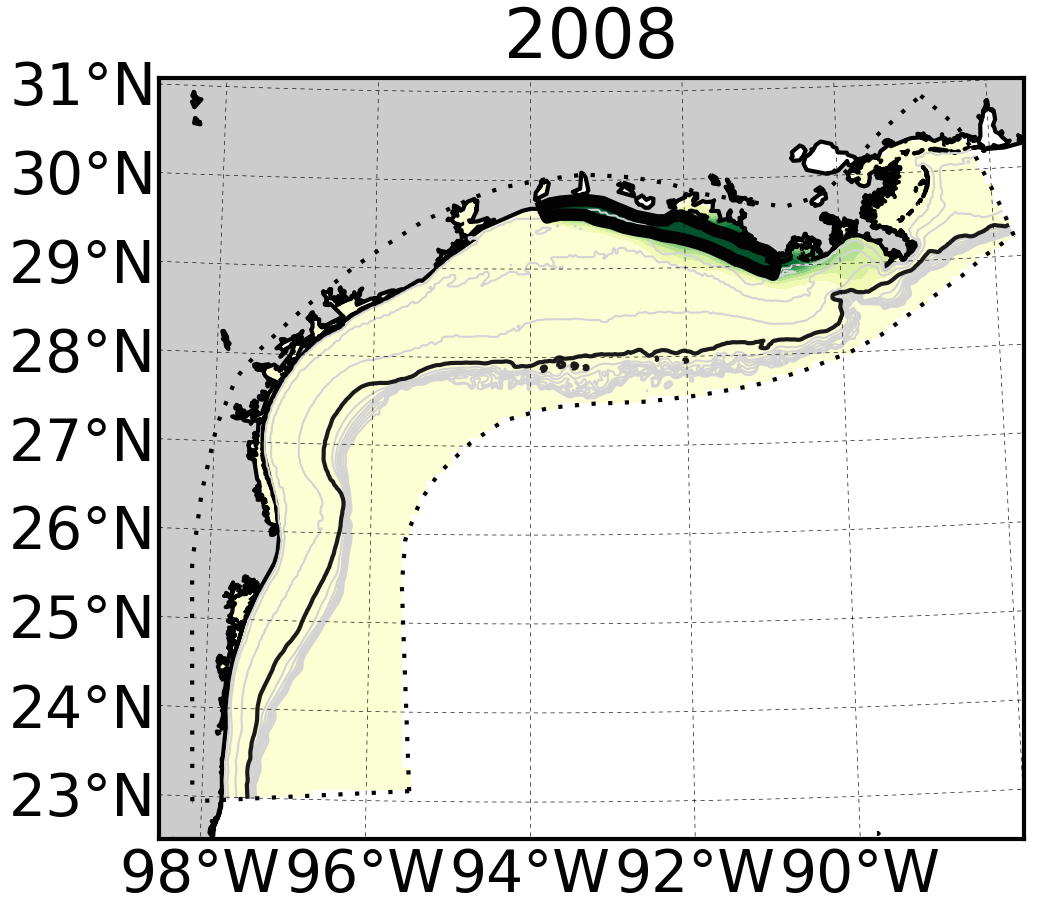
\includegraphics[width=0.65\textwidth]{figures/coastCHinterannual-winter_2008}}
		\only<2>{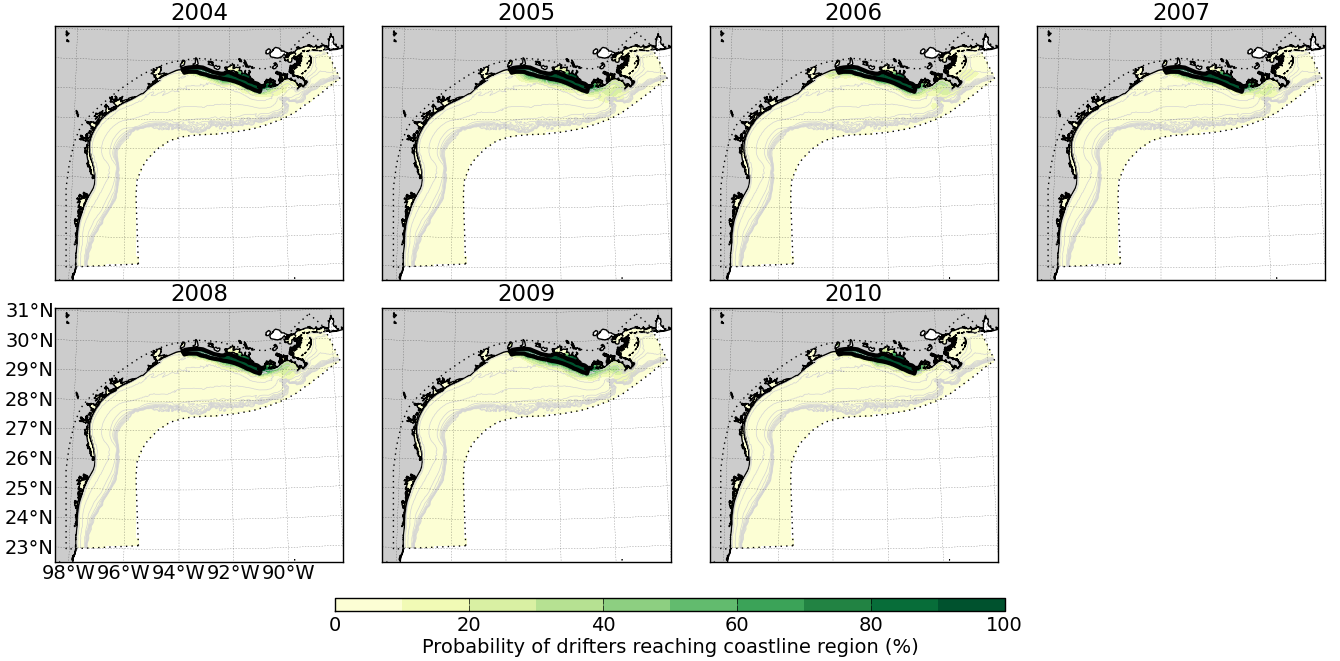
\includegraphics[width=\textwidth]{figures/coastCHinterannual-winter}}
	\end{figure}
\end{frame}
\begin{frame}[t]\frametitle{Coastline connectivity: South Texas}
	\begin{figure}[htbp]
		\centering
		\only<1>{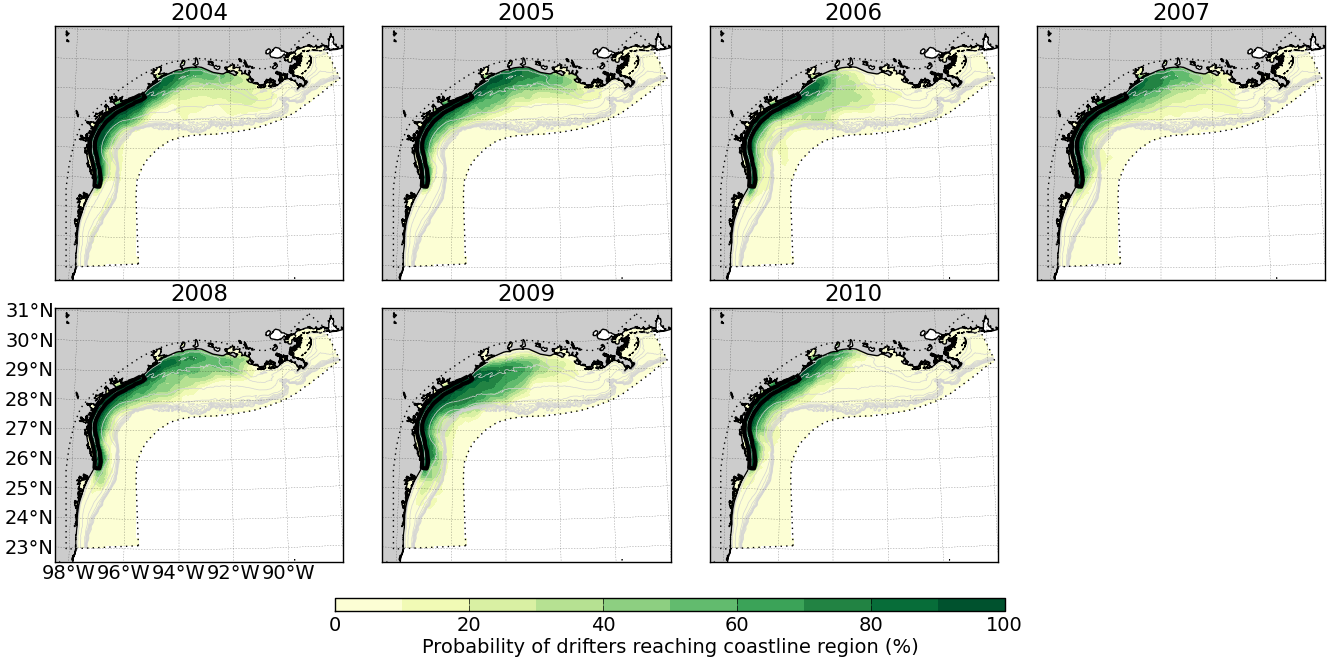
\includegraphics[width=\textwidth]{figures/coastSTXinterannual-winter}}
		% \only<2>{\includegraphics[width=\textwidth]{figures/coastSTXinterannual-winter_wind}}
	\end{figure}
\end{frame}

\begin{frame}[t]\frametitle{Error due to temporal sampling}
	\begin{figure}[htbp]
		\centering
		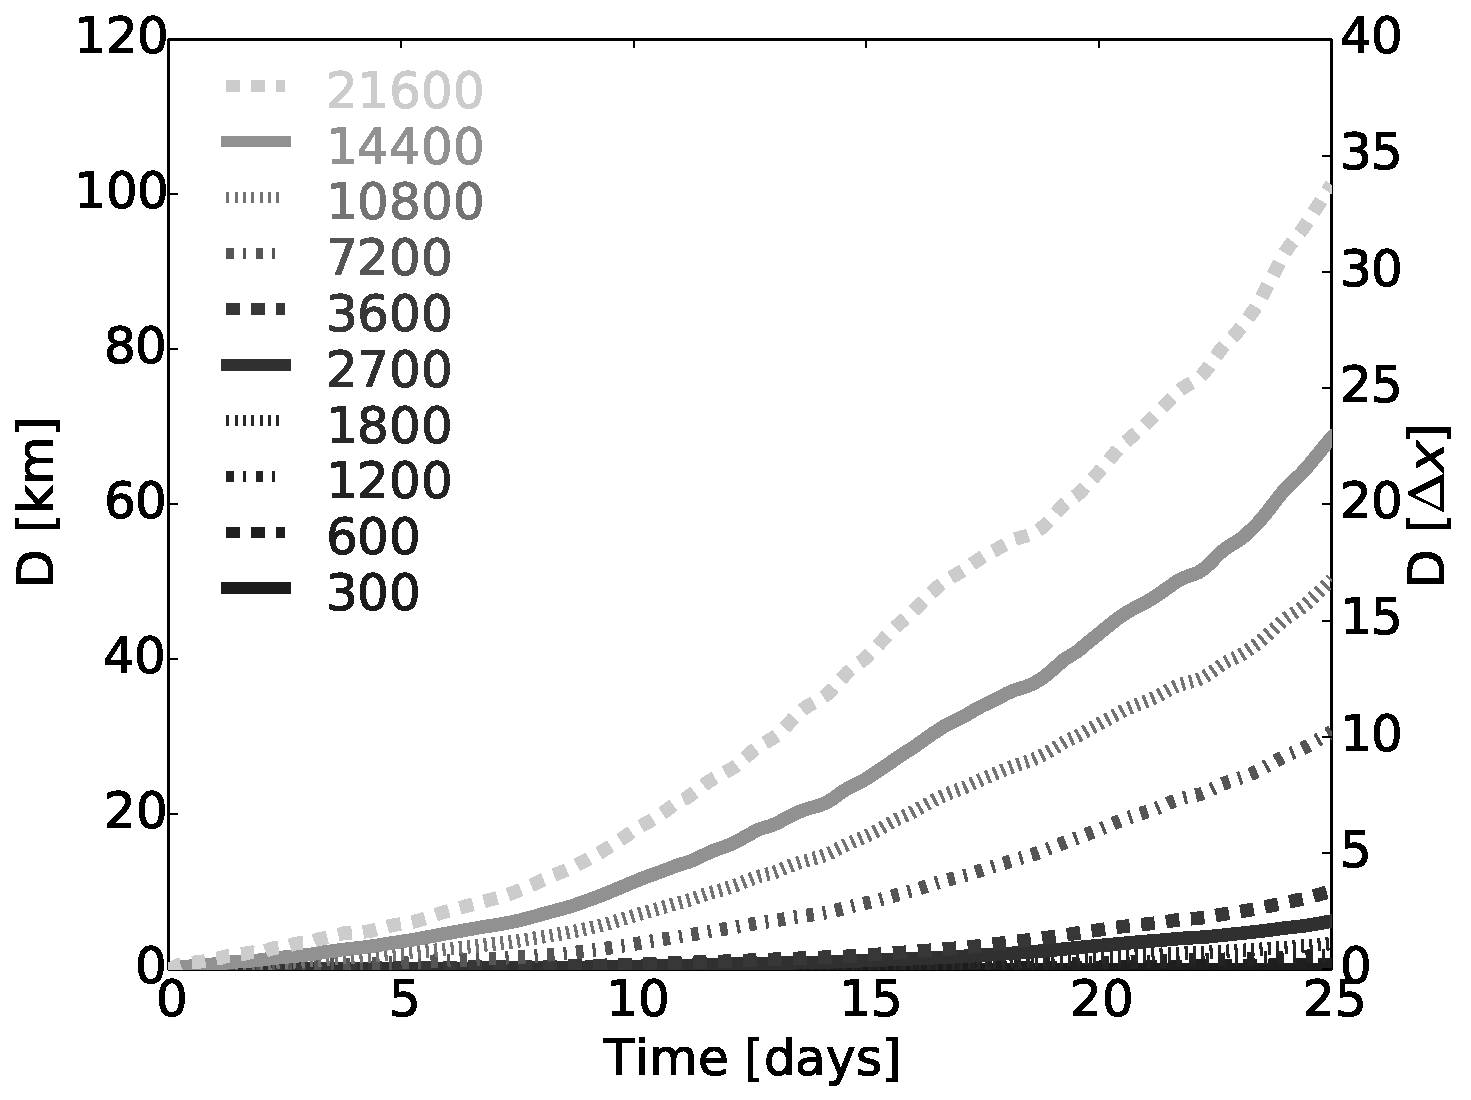
\includegraphics[width=0.8\textwidth]{figures/D}
	\end{figure}
\end{frame}

\begin{frame}[t]\frametitle{River tracks}
	\begin{figure}[htbp]
		\centering
		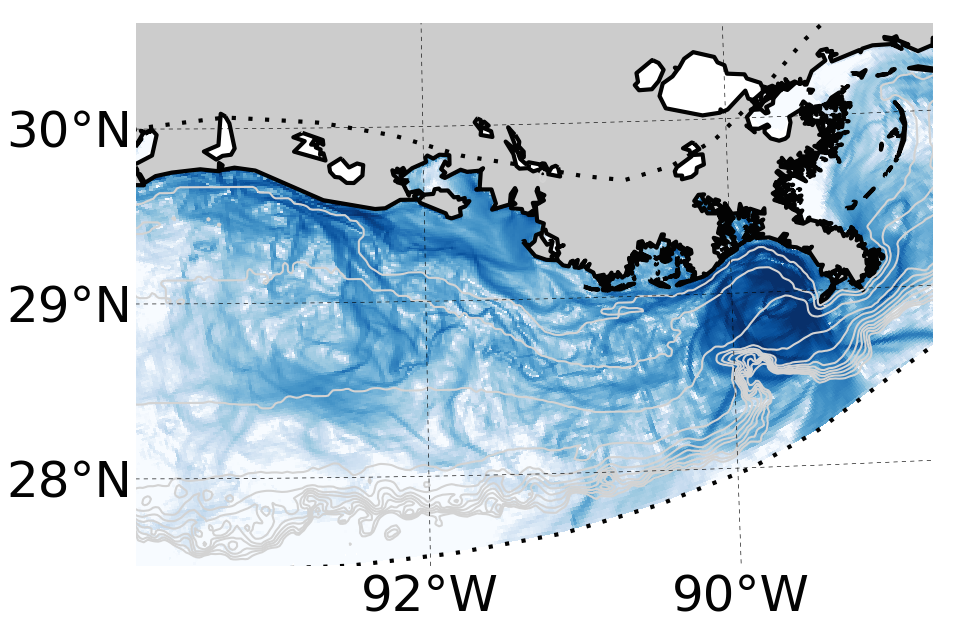
\includegraphics[width=0.9\textwidth]{figures/river_drifter_tracks}
	\end{figure}
\end{frame}

\section{Summary}

\begin{frame}[t]\frametitle{Summary}
    \begin{itemize}
    	\item {\Large Simulated drifter tracks improve understanding of transport processes}
    	\item[] ~
    	\item {\Large Many coastal concerns are transport-based}
    	\item[] ~
    	\item {\Large TracPy wraps trajectory model TRACMASS}
    	\item[] ~
    	\item {\Large Code has been used for several applications so far}
    	\item[] ~
    	% \item {\Large Forcing mechanisms have seasonal trends that substantially affect transport}
    	% \item[] ~
    	% \item {\Large Small differences in trends can lead to distinct connectivity patterns in different years}
    	% \item[] ~
    	\item {\Large Improved understanding can help address coastal issues}
    	% \item[] ~
    \end{itemize}
\end{frame}


% Funding, with logos
\begin{frame}
	\frametitle{Thank you!}
	\begin{figure}[htbp]
		\centering
		\subfigure{
\includegraphics[width=.45\textwidth]{figures/TAM-Logo.png}}
		\subfigure{
\includegraphics[width=.45\textwidth]{figures/gisr}}
	\end{figure}
\end{frame}

% \appendix

% \begin{frame}[t,noframenumbering]\frametitle{Seasonal: Cross-shelf transport: Shelf eddies}
% 	\vskip4ex
% 	\begin{figure}[htbp]
% 		\centering
% 		\includegraphics[width=0.8\textwidth]{figures/dispersion_diagram1}
% 	\end{figure}
% \end{frame}
% \begin{frame}[t,noframenumbering]\frametitle{Seasonal: Cross-shelf transport: Shelf eddies}
% 	\vskip4ex
% 	\begin{figure}[htbp]
% 		\centering
% 		\includegraphics[width=0.8\textwidth]{figures/dispersion_diagram2}
% 	\end{figure}
% \end{frame}
% \begin{frame}[t,noframenumbering]\frametitle{Seasonal: Cross-shelf transport: Shelf eddies}
% 	\vskip4ex
% 	\begin{figure}[htbp]
% 		\centering
% 		\includegraphics[width=0.8\textwidth]{figures/dispersion_diagram3}
% 	\end{figure}
% \end{frame}
% \begin{frame}[t,noframenumbering]\frametitle{Seasonal: Cross-shelf transport: Shelf eddies}
% 	\vskip4ex
% 	\begin{figure}[htbp]
% 		\centering
% 		\includegraphics[width=0.8\textwidth]{figures/D2}
% 	\end{figure}
%     {\tiny data from LaCasce \& Ohlmann (2003), Journal of Marine Research}
% \end{frame}


\end{document}